% !TeX root = ../thuthesis-example.tex

% \chapter{研究方法}
\chapter{基于多模态的动态手势识别算法研究}
\label{sec:GR}
针对动态手势识别中“信息冗余(IR)”和 “信息缺失(IA)”的挑战,如图~\ref{fig:MDSI} 所示,我们提出了一种用于 RGB-D 手势识别的新型可插拔方法,称为多策略解耦和语义集成网络 (MDSI)。所提出的可插拔式 MDSI 方法的总体框架如图 \ref{fig:MDSI} 所示。为了解决信息冗余 (IR) 问题,我们引入了多策略解耦网络 (MDN),通过“姿势-运动”和“空间-时间-通道”解耦来强调不同尺度与不同维度的特征信息 (第~\ref{sec:MDN}节)。
为了解决信息缺失 (IA) 问题,我们提出了一个语义集成网络 (SIN),它有两个关键组件:语义滤波器 (SF) 和语义标签平滑 (SLS),以补充手势识别中缺失的信息 (第~\ref{sec:SIN}节)。
%应用
\begin{figure}[tb]
  \centering
  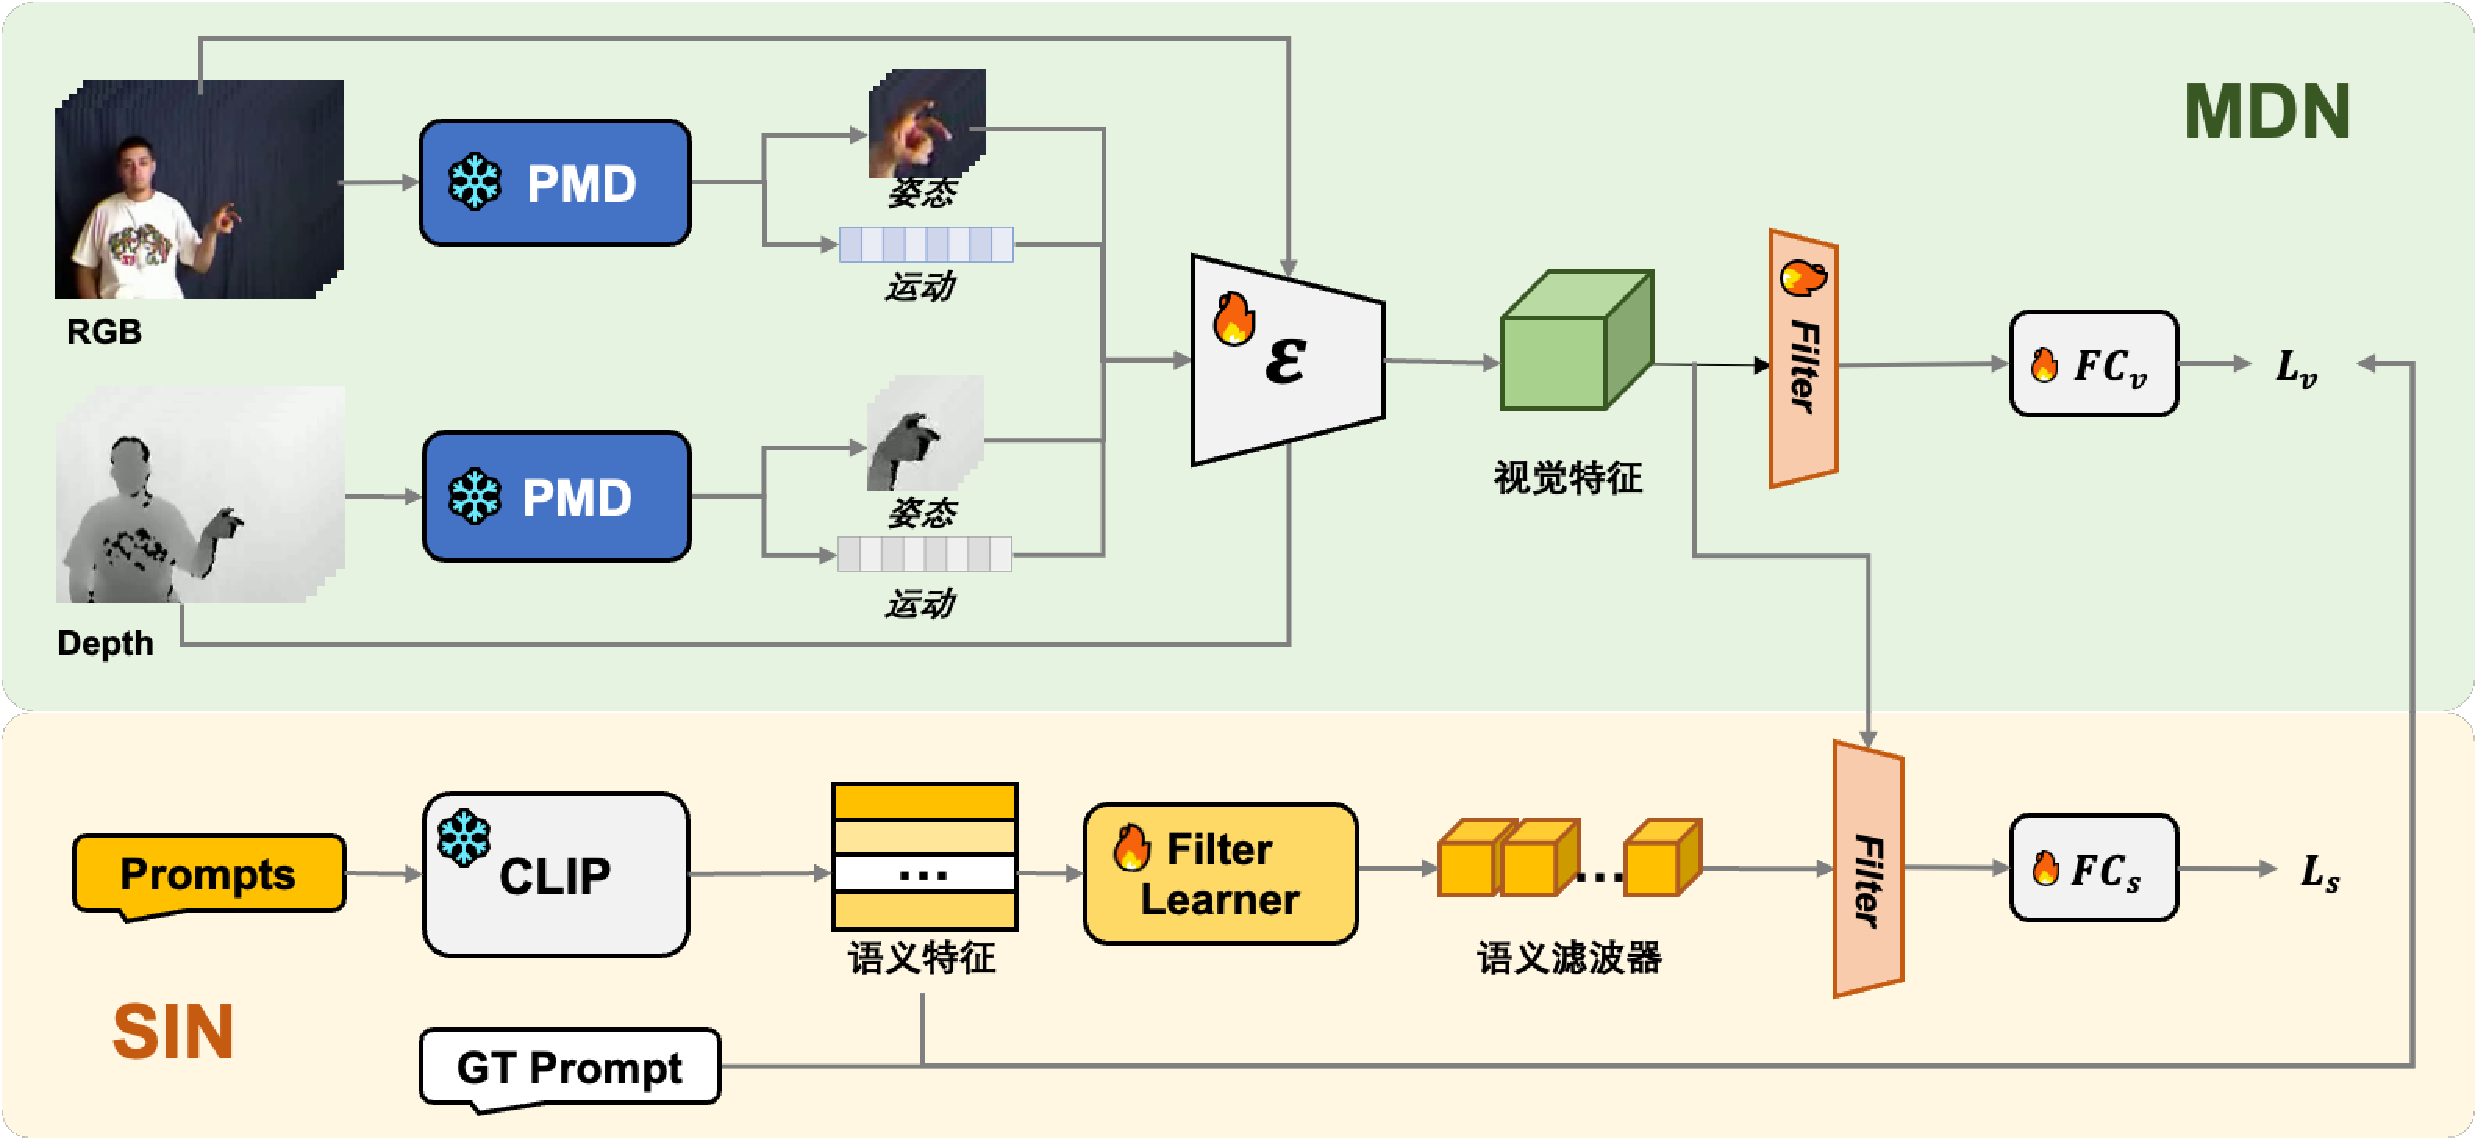
\includegraphics[width=\linewidth]{MDSI_v1.2.pdf}%framework.png}
  \caption{我们的可插入式多策略语义集成解耦 (MDSI) 框架概述。MDSI 可以无缝集成到基本编码器 $\varepsilon$ 中,从两个方面增强手势识别性能:
  i) 对于信息冗余,MDN (图~~\ref{fig:MDN}) 通过 PMD 和 STCD 强调不同维度和尺度的特征信息 (图~\ref{fig:handdecomp})。
  ii) 对于信息缺失,SIN 通过 SF 将自然语言建模与 SLS 一起集成到手势识别中 (图~\ref{fig:SIN})。}
  \label{fig:MDSI}
\end{figure}

\section{多策略手势特征解耦网络}
\label{sec:MDN}
\begin{figure}[tb]
  \centering
  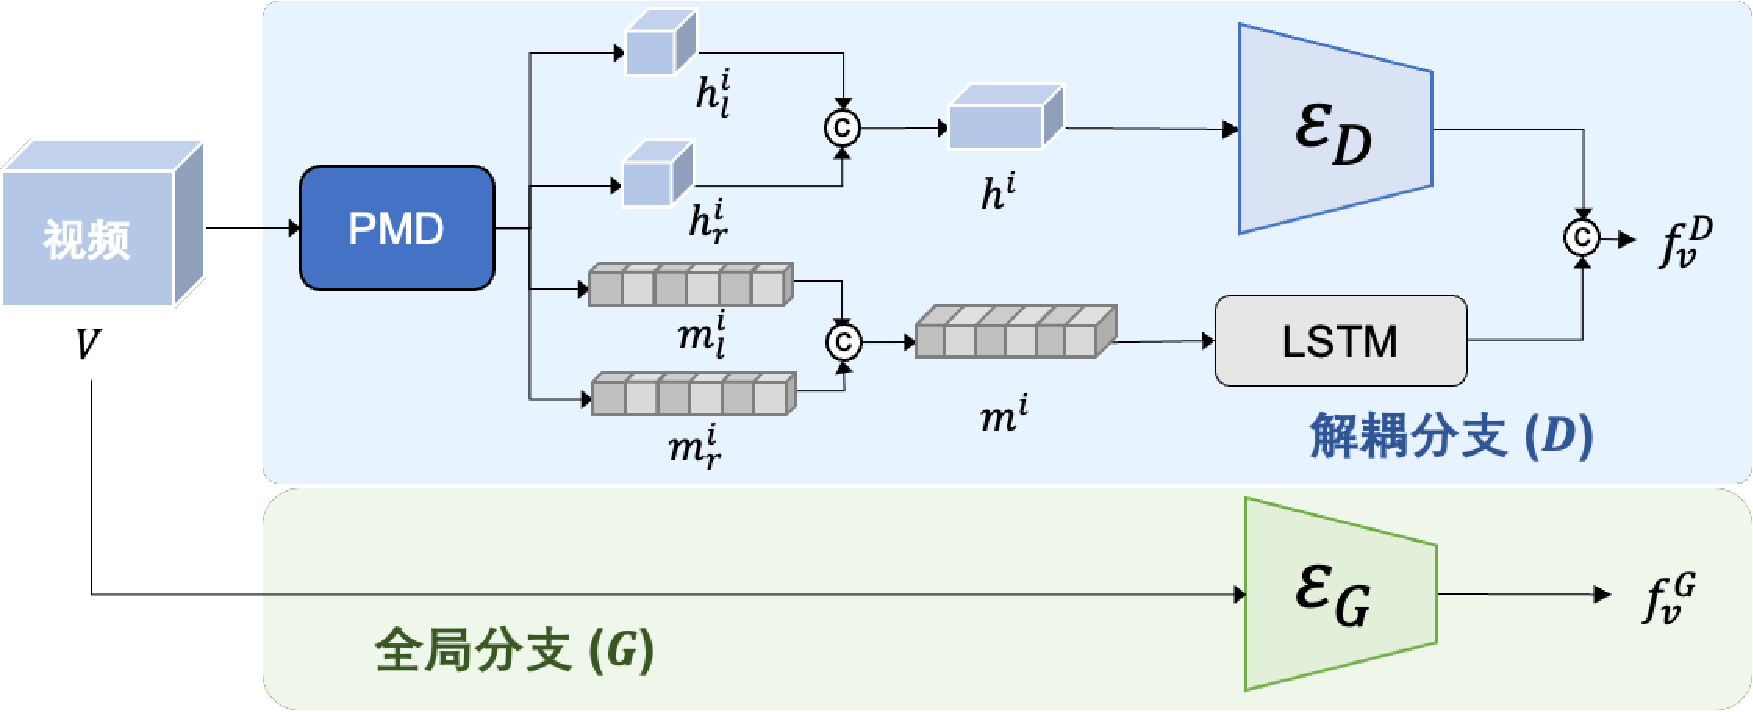
\includegraphics[width=0.8\linewidth]{MDN_v1.pdf}
    \caption{多策略解耦网络 (MDN)。MDN 配置为双分支视频编码器。i) 全局分支 ($\mathcal{G}$) 将原始视频 $\mathbf{V}$ 作为输入并对全局特征进行编码。ii) 解耦分支 ($\mathcal{D}$) 利用 PMD 模块同时捕获解耦的细粒度姿势 $\mathbf{h}$ 和粗粒度手部运动 $\mathbf{m}$。iii) STCD 模块插入编码器 $\varepsilon_{\mathcal{G}}$ 和 $\varepsilon_{\mathcal{D}}$ 的不同阶段,以执行与维度无关的解耦和注意。}
  \label{fig:MDN}
\end{figure}

在本节中,我们介绍了一种多策略解耦网络 (MDN),它配置为双分支架构,包括姿势-运动解耦模块 (PMD) 和空间-时间-通道解耦模块 (STCD)。
如图~\ref{fig:MDN} 所示,我们首先利用 PMD 将手势视频 $\mathbf{V}$ 解耦为细粒度姿势 $\mathbf{h}$ 和粗粒度运动 $\mathbf{m}$。原始视频 $\mathbf{V}$ 以及解耦结果 $\mathbf{(h, m)}$ 通常分别输入到 MDN 的全局分支 ($\mathcal{G}$) 和分解分支 ($\mathcal{D}$) 进行视觉时空特征提取。
此外,可插入 STCD 插入编码器 $\varepsilon_{\mathcal{G}}$ 和 $\varepsilon_{\mathcal{D}}$ 的各个阶段,以实现有效的与维度无关的解耦和注意。

\subsection{姿态-运动解耦(PMD)}
\label{sec:pose-motion}
\begin{figure}[tb]
\centering
\subcaptionbox{\label{fig:PMD}}
{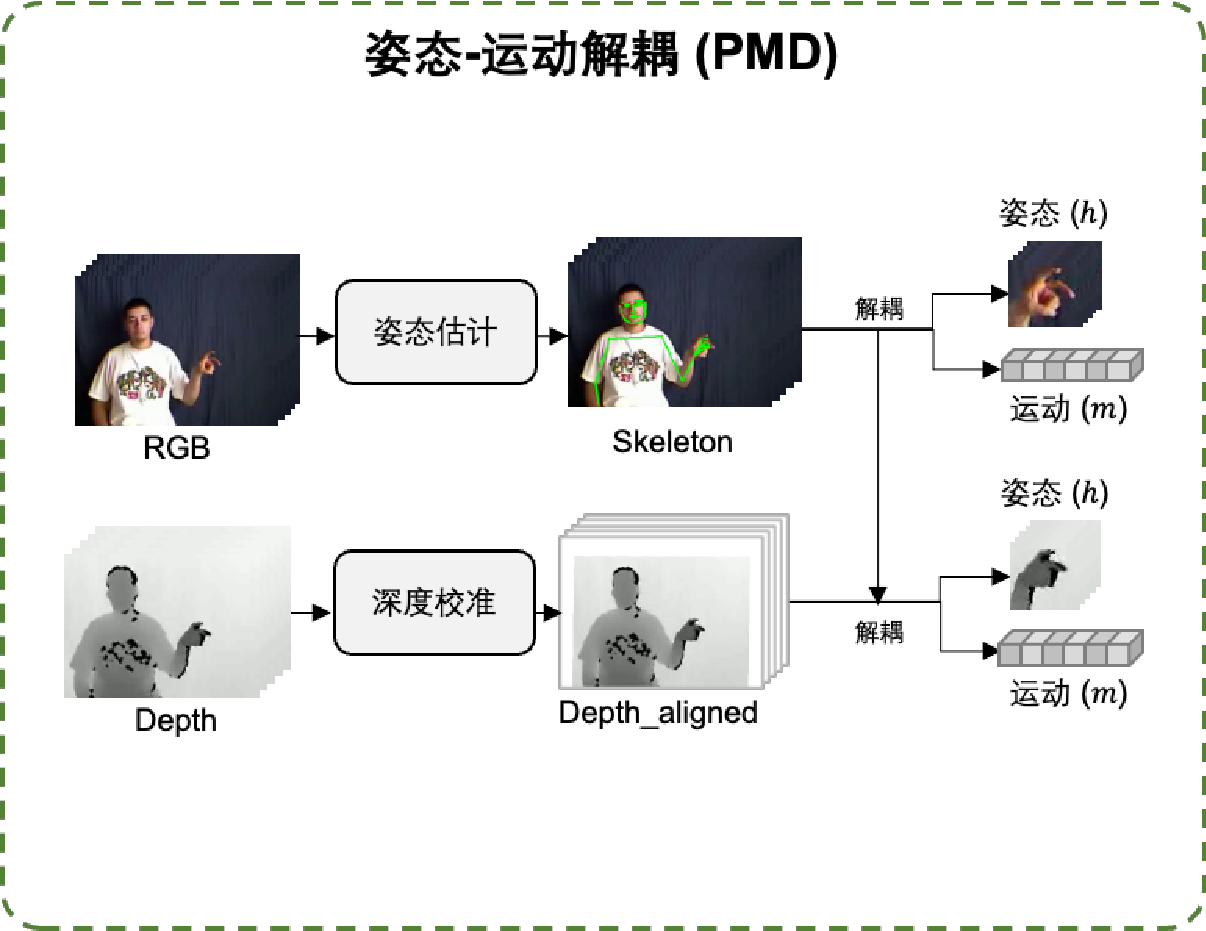
\includegraphics[width=0.44\linewidth]{PMD.pdf}}
\subcaptionbox{\label{fig:STCD}}
{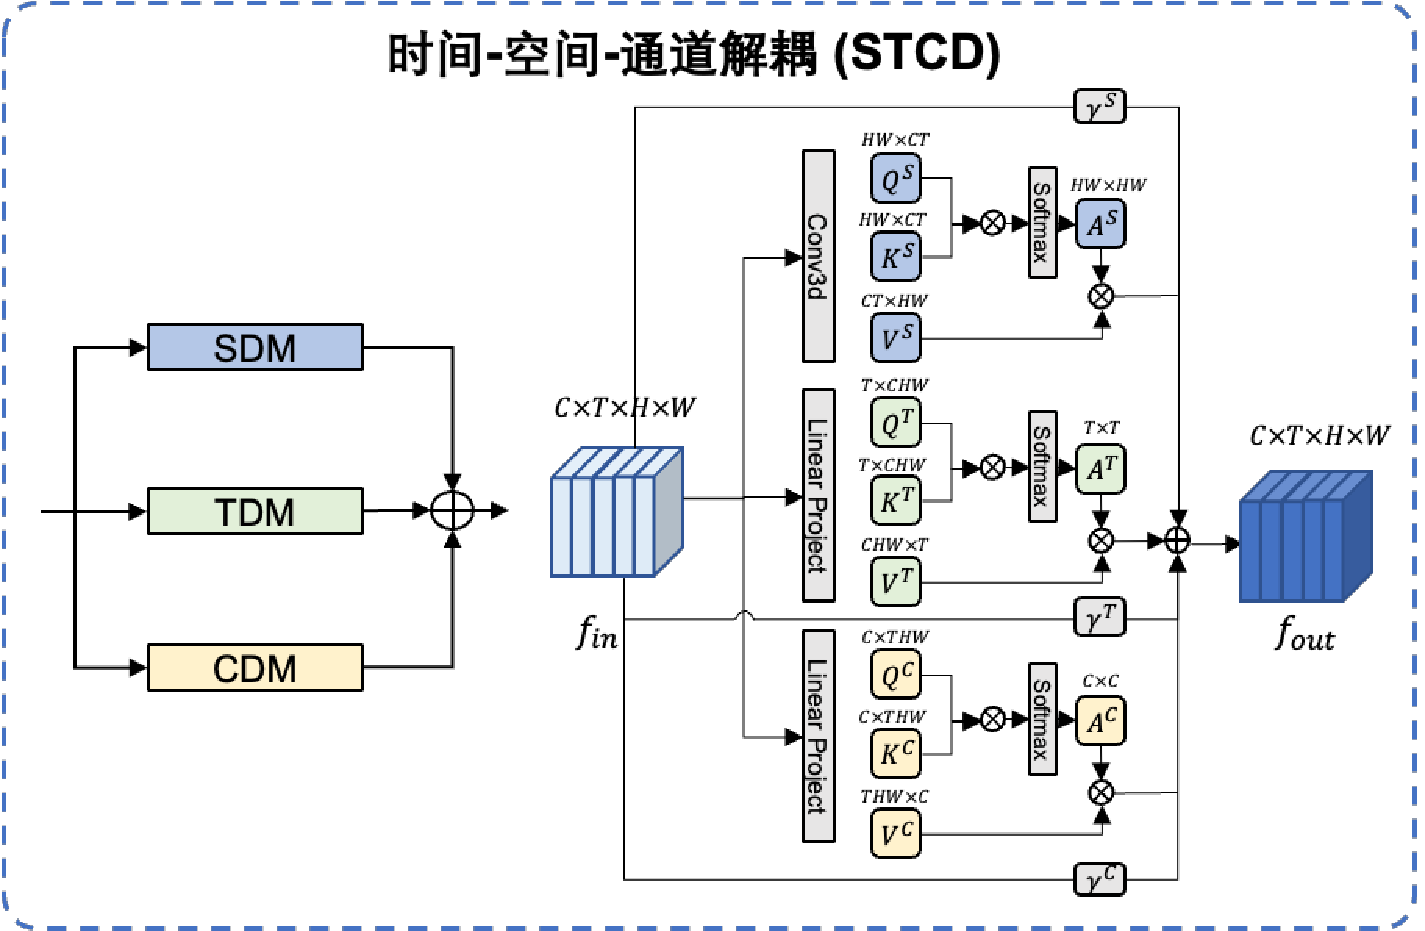
\includegraphics[width=0.52\linewidth]{STCDv1 .pdf}}
\caption{多策略解耦管道。 (a) 姿势-运动解耦 (PMD),(b) 空间-时间-通道解耦 (STCD)。}
\label{fig:handdecomp}
\end{figure}

如图~\ref{fig:PMD}所示,PMD 主要包括三个阶段:i) 姿势估计、ii) 深度校准和 iii) 姿势-运动解耦。
对于 RGB 数据,我们首先使用在 COCO-WholeBody 数据集 \cite{jin2020whole} 上预训练的姿势估计器 HRNet \cite{sun2019deep} 来提取并保存每帧 2D 身体骨架\footnote{请注意,姿势估计器在训练期间处于冻结状态,确保它不会引入任何额外的计算成本。此外,使用手部检测器检测和分割手部是现场的常见做法 \cite{AVOLA2022108762,zhou2021regional,chen2022multi},这是一个完全公平的设置。}。
对于深度数据,我们提前进行视频校准以确保配准 \cite{liu2017continuous}。
具体来说,对于 IsoGD 数据集 \cite{wan2016chalearn},我们利用 Liu 等人提供的对齐深度视频数据 \cite{liu2017continuous},并进一步调整 Narayana 等人提供的深度数据映射 \cite{narayana2018focus},使用以下变换:$D'=\frac{D-7}{0.93}-14$。
对于 THU-READ 数据集,深度数据已提前校准。
对齐良好的深度数据可以采用从 RGB 视频中提取的相同骨架进行后续操作。

我们利用提取的骨架数据将原始视频 $\mathbf{V}$ 分解为手部姿势 $\mathbf{h}$ 和手部运动 $\mathbf{m}$。
首先,给定第 $i$ 帧的骨架数据 ($i \in 0, 1, ..., T$),我们分别过滤每只手的 22 个关键点并描绘出最小手部边界框。
随后,我们裁剪缩放后的边界框(比例=1.2)以获得表示细粒度姿势 $\mathbf{h}^{i}$ 的裁剪手部图像。为了公式化粗粒度运动向量$\mathbf{m}^{i} \in \mathbb{R}^{8}$,我们将边界框的 8 个位置属性堆叠如下:$\mathbf{m}^{i} = \left[e^{i}, x^{i}_{min}, y^{i}_{min}, x^{i}_{max}, y^{i}_{max}, w^{i}, h^{i}, r^{i}\right]^{\top}$,其中 $e^{i} \in \{0, 1\}$ 表示相应的手是否出现在第 $i$ 帧%(参见 Eq.~\ref{eq:e})
,$\{x^{i}_{min}, y^{i}_{min}\}$ 和 $\{x^{i}_{max}, y^{i}_{max}\}$ 为边界框左上角和右下角顶点的坐标,$w^{i}, h^{i}$ 分别对应宽和高,$r^{i}=w^{i}/h^{i}$ 表示长宽比。
为了区分左右手,上述操作分别在每只手上独立执行,然后连接起来,得到最终的解耦特征:$\mathbf{h}^{i} = \left[\mathbf{h}^{i}_l, \mathbf{h}^{i}_r\right]$,$\mathbf{m}^{i} = \left[\mathbf{m}^{i}_l, \mathbf{m}^{i}_r\right]$。
具体来说,$\mathbf{h}$ 和 $\mathbf{m}$ 分别在宽度方向和通道方向连接。

此外,为了减轻姿势估计不准确的影响,我们设计了一个 \emph{分割验证机制}:检测到的关键点置信度低且关键点数量较少的骨架被标记为错误检测,并且相应的姿势特征 $\mathbf{h}^{i}$ 被分配零值。%\textcolor{red}{更多详细信息请参阅 \ref{sec:appendix_pmd}。}

\subsection{空间-时间-通道解耦 (STCD)}
\label{sec:STCD}
鉴于手势识别中存在紧密耦合的时空冗余\cite{zhou2023unified},我们引入了 STCD(图 ~\ref{fig:STCD}),它配置了三个包含注意机制的独立于维度的模块:i) 空间解耦模块 (\textbf{SDM})、ii) 时间解耦模块 (\textbf{TDM}) 和 iii) 通道解耦模块 (\textbf{CDM})。
以$\varepsilon$中提取的输入中间特征图$\mathbf{f}_{in}\in \mathbb{R}^{C\times T\times H\times W}$作为输入,该框架帮助网络有效滤除各个维度上的冗余信息,输出优化的特征图$\mathbf{f}_{out}\in \mathbb{R}^{C\times T\times H\times W}$,从而帮助训练。

以 SDM 为例,其目的是识别每帧手势特征中的关键空间区域。首先,给定 $\mathbf{f}_{in}$,我们使用 Conv3d 来导出查询、键和值特征,分别表示为 $\mathbf{Q}^{\mathcal{S}}$、$\mathbf{K}^{\mathcal{S}}$ 和 $\mathbf{V}^{\mathcal{S}}$。
我们合并时间和通道维度以获得 \emph{空间} 查询、键和值向量:$\mathbf{q}^{\mathcal{S}}\in \mathbb{R}^{HW\times CT}$、$\mathbf{k}^{\mathcal{S}}\in \mathbb{R}^{HW\times CT}$、$\mathbf{v}^{\mathcal{S}}\in \mathbb{R}^{CT\times HW}$。
然后,利用 $\mathbf{q}^{\mathcal{S}}$ 和 $\mathbf{k}^{\mathcal{S}}$ 计算注意矩阵 $\mathbf{A}^{\mathcal{S}}\in \mathbb{R}^{HW\times HW}$,如下所示:

\begin{equation}
\mathbf{A}^{\mathcal{S}} = \text{softmax}\left(\mathbf{q}^{\mathcal{S}}\left(\mathbf{k}^{\mathcal{S}}\right)^{\top}\right).
\end{equation}
随后,空间注意力向量 $\mathbf{f}^{\mathcal{S}}\in \mathbb{R}^{CT\times HW}$ 可以通过以下公式计算:
\begin{equation}
\mathbf{f}^{\mathcal{S}} = \mathbf{v}^{\mathcal{S}} \mathbf{A}^{\mathcal{S}}.
\end{equation}
我们恢复时间和通道维度以获得空间注意特征图$\mathbf{f}'^{\mathcal{S}}\in \mathbb{R}^{C\times T\times H\times W}$。
此外,为了促进网络收敛并调节网络注意力水平,我们引入了可学习的残差连接。最终的空间优化特征$\mathbf{f}_{out}^{\mathcal{S}}$可以按如下方式计算:$\mathbf{f}_{out}^{\mathcal{S}} = \gamma^{\mathcal{S}} \mathbf{f}'^{\mathcal{S}} + \mathbf{f}_{in}$,
其中$\gamma^{\mathcal{S}}$是SDM的可学习残差权重。

TDM 和 CDM 分别关注手势特征中的关键帧和通道,其操作与 SDM 类似。
此外,STCD 的结果输出被表达为三个解耦模块输出的聚合。
具体而言,我们设计了一个并行范式 (图 ~\ref{fig:STCD})
STCD 的结果输出 ${f}_{out}$ 可以表示如下:$\mathbf{f}_{out} = \mathbf{f}_{out}^{\mathcal{S}} + \mathbf{f}_{out}^{\mathcal{T}} + \mathbf{f}_{out}^{\mathcal{C}}$。

\subsection{双分支视频编码器}
\label{sec:DBVE}
如图~\ref{fig:MDN}所示,MDN 配置有两个分支:i) \emph{全局分支} ($\mathcal{G}$) 将原始视频 $\mathbf{V}$ 作为特征提取和识别的输入;ii) \emph{解耦分支} ($\mathcal{D}$) 利用解耦后的特征 $\mathbf{(h, m)}$ 作为输入,同时捕获细粒度的手势姿势变化和粗粒度的手部运动。
我们为每个分支配置一个视频编码器 $\varepsilon$。
此外,我们在 $\mathcal{D}$ 分支中引入了一个长短期记忆 (LSTM) 模型,用于运动建模(图~\ref{fig:MDN})。
特征提取过程可以表述如下:
\begin{equation}
\label{eq:fv}
\begin{aligned}
  \mathbf{f}_{v}^{\mathcal{G}} &= \Phi_{\mathcal{G}}(\mathbf{V}), \\
  \mathbf{f}_{v}^{\mathcal{D}} &= \Phi_{\mathcal{D}}(\mathbf{h}, \mathbf{m}).
\end{aligned}
\end{equation}
其中$\Phi_{\mathcal{G}}$表示$\mathcal{G}$分支网络,$\Phi_{\mathcal{D}}$表示$\mathcal{D}$分支网络。
得到的视觉特征$\mathbf{f}_{v}^{\mathcal{G}}, \mathbf{f}_{v}^{\mathcal{D}}$将分别输入到下面的SIN网络中进行语义集成。

\begin{figure}[tb]
\centering
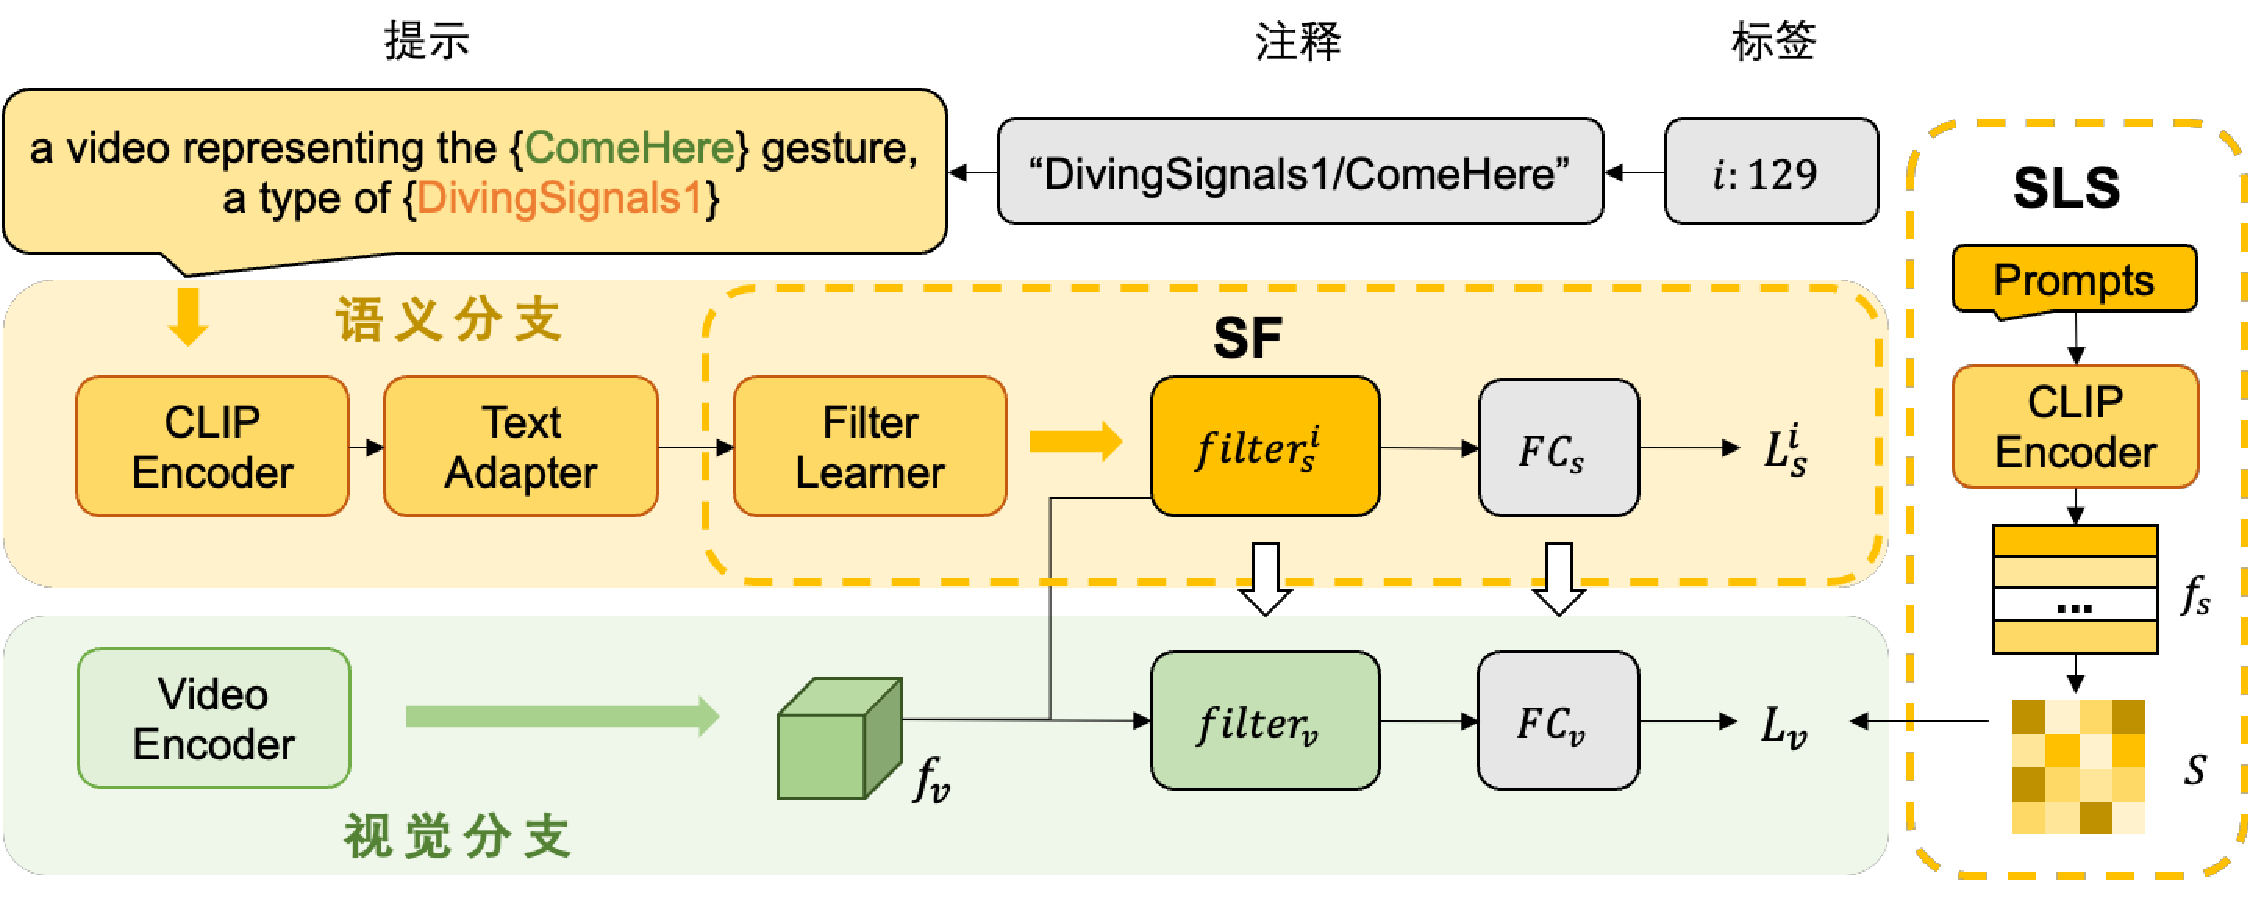
\includegraphics[width=1.0\linewidth]{SIGRv1 .pdf}
\caption{语义整合网络 (SIN) 结合了语义滤波器 (SF) 和语义标签平滑 (SLS),以促进语义知识整合。 }
\label{fig:SIN}
\end{figure}
\section{多模态手势语义集成网络}
\label{sec:SIN}
手势识别中的信息缺失挑战(第~\ref{sec:intro}节)激励我们结合自然语义信息作为指导。
所提出的语义集成网络 (SIN)(如图~\ref{fig:SIN} 所示)由两个分支组成:i) \emph{semantic} 分支,以语义嵌入和语义滤波器 (SF) 为特色;ii) \emph{vision} 分支,以语义标签平滑 (SLS) 为辅助。

\subsection{语义嵌入}
如图~\ref{fig:SIN}所示,鉴于手势数据集 \cite{wan2020chalearn,tang2017action,molchanov2016online} 通常使用类索引作为标签,我们首先生成与手势标签相对应的语义提示。具体来说,我们编译语义注释并设计提示(prompt),以强调每个手势数据集的独特特征。
然后,我们利用预训练的 CLIP 的文本编码器 \cite{radford2021learning} 和适配器 \cite{gao2024clip} 生成和细化深度语义嵌入 $\mathbf{f}_{s}\in \mathbb{R}^{N\times 1024}$($N$ 表示类数)。%\textcolor{red}{有关进一步的实施细节,请参阅 \ref{sec:appendix_se}。}

\subsection{语义滤波器 (SF)}
从动态卷积技术中汲取灵感~\cite{yang2019condconv,chen2020dynamic},我们引入了语义滤波器 (SF),用于通过卷积混合多模态特征。%(有关更多详细信息,请参阅 \ref{sec:appendix_SF})。

我们引入一个线性\emph{Filter Learner}(图~\ref{fig:SIN})来导出语义滤波器。
设语义滤波器的数量为$n$,以相应的$n$个语义嵌入$\mathbf{f}_{s} \in \mathbb{R}^{n\times 1024}$为输入,通过线性映射输出语义滤波器参数$\mathbf{f'}_{s}\in \mathbb{R}^{n\times N_p}$,然后将这些参数重塑为$n$个语义滤波器$\boldsymbol{\Theta}_{s}\in \mathbb{R}^{n\times c\times k^{d_k}}$,其中每个滤波器$\boldsymbol{\Theta}_{s}^i$代表一个卷积核。
第 $i$ 个滤波器 $\boldsymbol{\Theta}_{s}^i$ 的参数数量定义为:$N_p=c\times k^{d_k}$,其中 $c$ 表示视觉特征 $\mathbf{f}_{v}$ 的输入通道(Eq.\ref{eq:fv}),$k$ 表示滤波器核大小(经验上设置为 3),$d_k$ 表示卷积维数(例如,对于 3d 卷积核,设置 $d_k=3$)。

随后,我们将每个 $\boldsymbol{\Theta}_{s}^i$(对应第 $a$ 个手势类别)作为过滤核,将视觉特征 $\mathbf{f}_{v}$(对应第 $b$ 个手势类别)作为输入,执行深度卷积。得到的每个混合语义特征 $\mathbf{f}_{SF}^i$ 可以表示为:
\begin{equation}
\mathbf{f}_{SF}^{i} = \text{Convolution}\left(\mathbf{f}_{v}, \boldsymbol{\Theta}_{s}^i\right),\quad i \in 1\dots n. \\
\end{equation}
这些混合语义特征被进一步激活和扁平化,通过全连接(FC)层生成语义分支识别结果。

为了监督语义分支的优化,我们将 \cite{zuo2023natural} 每个语义标签 $a$ 与样本视觉标签 $b$ 混合。
具体来说,语义分支的混合标签 $\mathbf{y}_{SF}^i \in \mathbb{R}^N$ 可以表示为:
\begin{equation}
y_{SF}^i[k] = \begin{cases}
1 & \text{如果 } k = a = b,\\
0.5 & \text{如果 } k = a \text{或 } k = b, a\neq b,\\
0 & \text{否则,}
\end{cases}
\end{equation}
其中 $y_{SF}^i[k]$ 表示 $\mathbf{y}_{SF}^i$ 的第 $k$ 个条目。
我们利用交叉熵损失来优化语义滤波器:
\begin{equation}
L_{s}^i = -\frac{1}{N}\sum_{k=1}^{N}{{y}_{SF}^i[k] \log\left(\hat{y}^i[k]\right)},
\end{equation}
同样,我们根据选定的 $n$ 个语义滤波器形成 $n$ 个混合标签,并获得相应的 $n$ 个语义预测。整体语义损失 $L_{s}$ 是 $n$ 个交叉熵损失的平均值:$L_{s} = \frac{1}{n}\sum_{i=1}^{n}{L_{s}^i}$。

如图~\ref{fig:SIN} 所示,为了捕获 SF 中嵌入的语义知识以进行 \textbf{推理},我们引入了一个与视觉滤波器 $\boldsymbol{\Theta}_{v}$ 类似的卷积核,遵循我们的视觉网络 MDN,并将语义分支的知识集成到视觉分支中。
具体而言,$\boldsymbol{\Theta}_{v}$ 和 $FC_{v}$ 分别通过其参数的加权和以及相应的 $\boldsymbol{\Theta}_{s}$ 和 $FC_{s}$ 的参数进行更新。
% 有关更多实施细节,请参阅 \ref{sec:appendix_hp}。

\subsection{语义标签平滑(SLS)}
与普通标签平滑 \cite{he2019bag} 相比,我们利用手势的语义相似性来生成有偏平滑标签,从而增强视觉分支识别视觉相似手势的能力。
具体来说,我们首先通过 CLIP 的文本编码器获取语义嵌入 $\mathbf{f}_{s} \in \mathbb{R}^{N\times 1024}$,然后使用余弦相似度 \cite{zuo2023natural} 构建提示相似度表 $\mathbf{S}$:$\mathbf{S} = \|\mathbf{f}_{s}\|_2\|\mathbf{f}_{s}\|_2^{\top} \in \mathbb{R}^{N\times N}$。
%
对于第 $b$ 个手势类别的训练样本,建议的平滑标签 $\mathbf{y}_{SLS}$ 可以表示为:
\begin{equation}
y_{SLS}[k] = \begin{cases}
1 - \sigma & \text{如果 } k = b,\\
\sigma \times \text{softmax}\left(S[b][k]/\tau\right) & \text{否则},
\end{cases}
\end{equation}
其中 $\sigma=0.2$,$\tau=0.5$。
类似地,交叉熵用于计算视觉分支损失:
\begin{equation}
L_{v} = -\frac{1}{N}\sum_{k=1}^{N}{y_{SLS}[k]\log\left(\hat{y}[k]\right)}. %SLS(\hat{y}_{vision},y)
\end{equation}

\subsection{整体损失}
整体损失是 $L_{s}$ 和 $L_{v}$ 的加权和:
\begin{equation}
Loss = w_{s} \times L_{s} + w_{v} \times L_{v}.
\label{eq:overall_loss}
\end{equation}
%
请注意,本文仅将 SIN 网络应用于每个全局视觉特征 $f_v^G$ (Eq.~\ref{eq:fv}),以确保视觉特征和语义特征之间交互的完整性。
因此,本文采用常用的分数融合方法来结合每个分支和模态的预测。

\section{实验结果与分析}
\label{sec:GR_EXP}
\subsection{实验设置}
\subsubsection{数据集}
我们在两个公共 RGB-D 手势数据集上评估了我们的方法:IsoGD \cite{wan2016chalearn} 和 THU-READ \cite{tang2017action}。它们都已被广泛使用,并且包含具有挑战性的场景。
IsoGD 数据集 \cite{wan2016chalearn} 收录了 47933 段 RGB-D 手势视频,由 21 位受试者完成 249 类手势动作。本文图 ~\ref{fig:samples} 展示了该数据集的示例样本。
此数据集中样本的背景多样性和手势相似性使其成为评估我们的方法对信息冗余 (IR) 和信息缺失 (IA) 影响的良好基准。
THU-READ 数据集 \cite{tang2017action} 包含 1920 个 RGB-D 自我中心手势视频,包含 8 个受试者执行的 40 个不同动作,由于细微的类内差异和背景噪音,这仍然具有挑战性。
为了进行评估,我们采用提供的留一法交叉验证协议 \cite{li2021trear}。

% 进一步地,我们利用奥比中光机器人平台(第~\ref{sec:robot}节)构建了自采数据集,并基于此评估了我们的方法。如图~\ref{fig:aobi_sample}所示,我们共采集了12类手势数据,每类包含25个样本。

% \begin{figure}
%   \centering
%   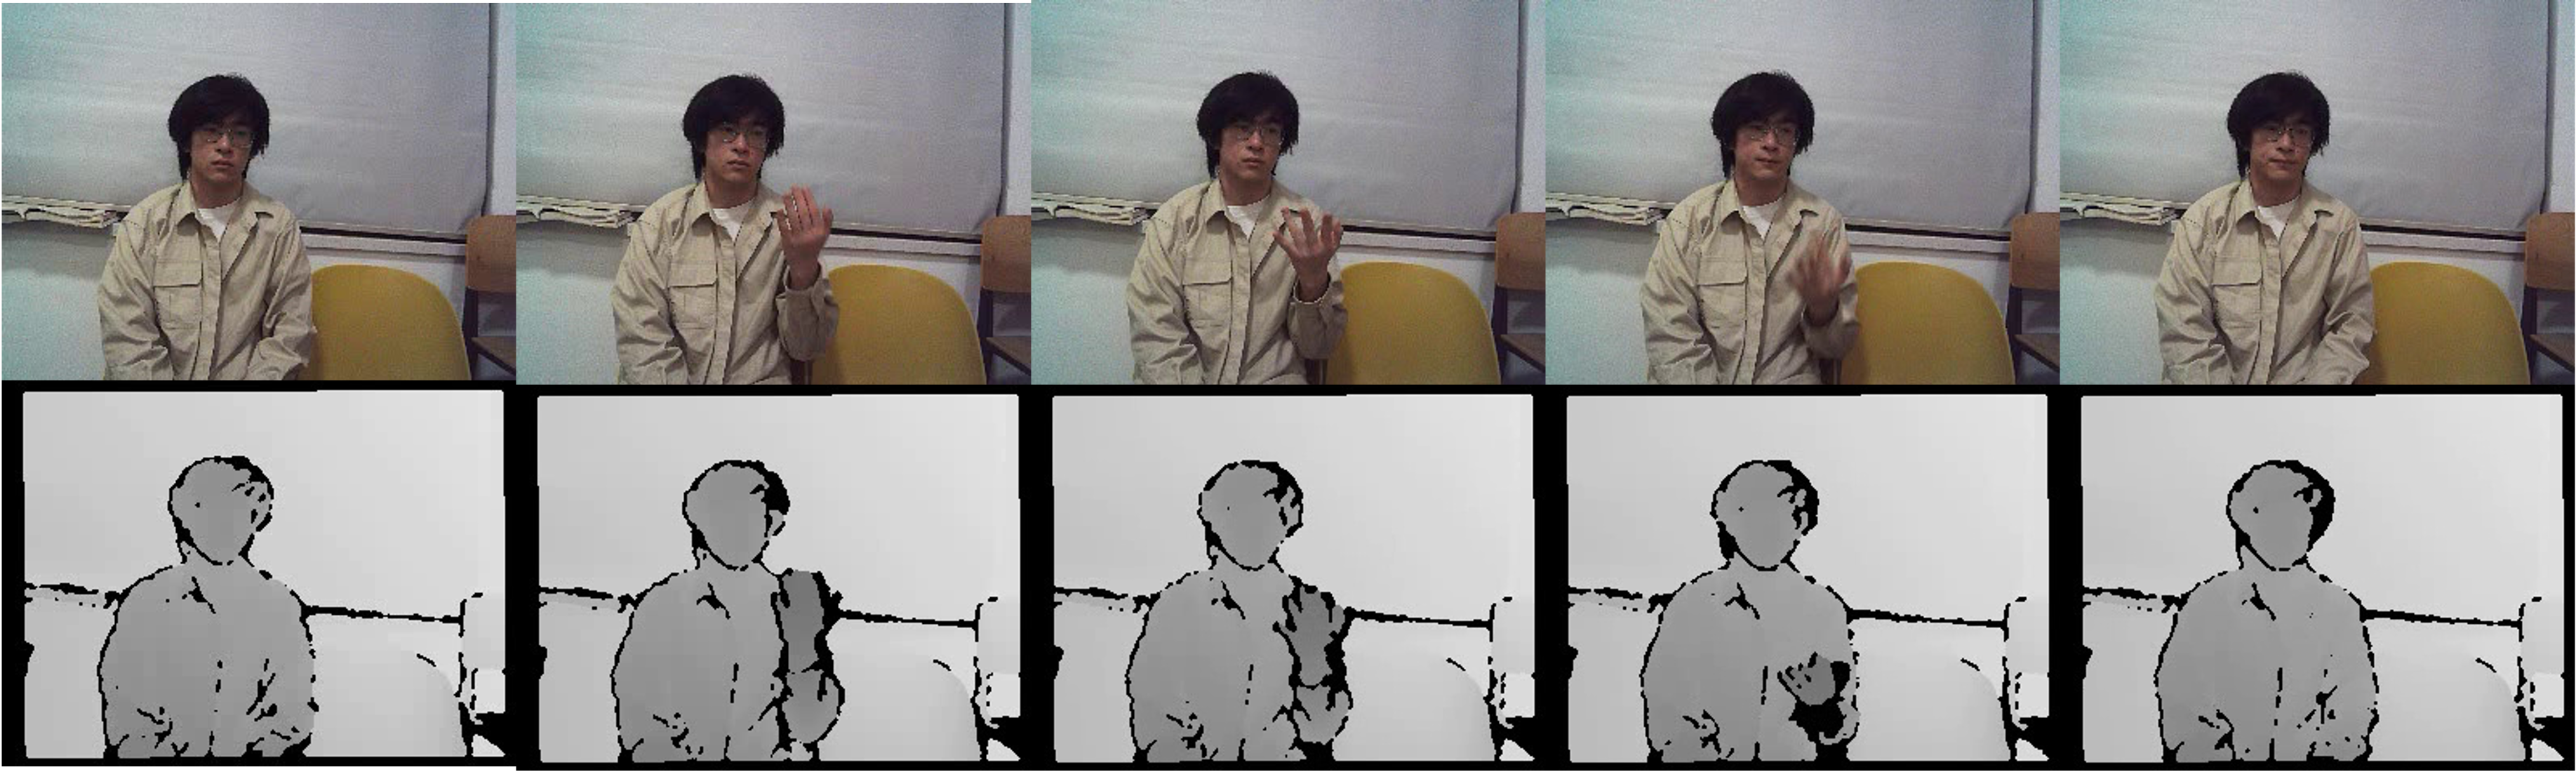
\includegraphics[width=0.8\linewidth]{aobi_sample.png}
%   % \caption*{}
%   \caption{机器人平台自采数据集样本示例}
%   \label{fig:aobi_sample}
% \end{figure}


\subsubsection{编码器骨干}
\label{sec:encoder_backbone}
我们实现了两个版本的 MDSI: \emph{MDSI-CNN} 和 \emph{MDSI-Transformer},分别将我们的可插拔方法集成到基于 CNN 的视频编码器 \cite{zhu2018continuous} 和基于 Transformer 的视频编码器 \cite{zhou2022decoupling} 中。这突出了 MDSI 的可插拔特性,使其能够集成到不同的编码器架构中。我们将这两个版本与最先进的方法进行比较,以验证我们的方法。

\subsubsection{实现细节}
\label{sec:implementation}
我们使用 Adam 作为优化器。
训练时,每个视频随机抽取32帧连续序列。原始输入序列随机裁剪至224 $\times$ 224像素,解耦的
手部序列调整至112 $\times$ 112像素。
数据增强包括空间裁剪、旋转、翻转和 Shufflemix+ \cite{zhou2023unified}。
与~\cite{yu2021searching,zhou2021regional,zhou2022decoupling,zhou2023unified} 类似,我们所有的实验都是在 20BN Jester V1 数据集上进行预训练的~\cite{materzynska2019jester}。
在推理过程中,输入序列被中心裁剪为 224 × 224。
我们根据视觉特征形状分别将 MDSI-CNN 和 MDSI-Transformer 的 SF 中的卷积维度 $d_k$ 设置为 3 和 1。
除非另有说明,所有消融研究均在 IsoGD 数据集的 RGB 数据上进行。
% 有关更多实施细节,请参阅 \ref{sec:appendix_hp}。

% \renewcommand{\arraystretch}{0.75}
% \setlength{\abovecaptionskip}{4pt}
% \setlength{\belowcaptionskip}{4pt}
% \setlength{\textfloatsep}{8pt}
\begin{table*}[htbp] %[!ht]
% \small
  \caption{与 IsoGD 数据集上最先进的方法的性能比较。最佳和第二佳方法通过 \textbf{加粗} 和 \underline{下划线}标注。}
    \centering
    \begin{tabular}{lccc}
    \toprule 
        {Modality} & {Backbone} &  {Methods}& {Accuracy(\%)} \\
     \midrule
        \multirow{9}*{RGB}& \multirow{5}*{CNN}  & ConvLSTMForGR~\cite{zhu2019redundancy}  & 57.42 \\ 
        ~&~& NAS~\cite{yu2021searching}  &  58.88 \\ 
        ~&~& RAAR3DNet~\cite{zhou2021regional} &  62.66 \\ 
        ~&~& MSA-3D~\cite{chen2022multi} & \underline{62.73} \\ 
        ~&~& \textbf{Ours} & \textbf{72.79} \\ 
        \cmidrule(lr){2-4}
        ~& \multirow{4}*{Transformer} & Decouple+Recouple~\cite{zhou2022decoupling} & 60.87 \\ 
        ~&~& MFST-Large~\cite{ma2023multi} & 61.26 \\ 
        ~&~& UMDR (32 frame)~\cite{zhou2023unified} & \underline{63.68} \\ 
        ~&~& \textbf{Ours} & \textbf{68.32} \\ 
     \midrule
     \midrule
        \multirow{9}*{Depth}& \multirow{5}*{CNN}  & ConvLSTMForGR~\cite{zhu2019redundancy} & 54.18 \\ 
        ~&~& NAS~\cite{yu2021searching} & 55.68 \\ 
        ~&~& RAAR3DNet~\cite{zhou2021regional} & 60.66 \\ 
        ~&~& MSA-3D~\cite{chen2022multi} & \underline{61.72} \\ 
        ~&~& \textbf{Ours} & \textbf{65.99} \\ 
        \cmidrule(lr){2-4}
        ~& \multirow{4}*{Transformer} & Decouple+Recouple~\cite{zhou2022decoupling}& 60.17 \\ 
        ~&~& MFST-Large~\cite{ma2023multi}& 61.29 \\ 
        ~&~& UMDR (32 frame)~\cite{zhou2023unified}& \underline{64.62} \\ 
        ~&~& \textbf{Ours} & \textbf{68.00} \\ 
     \midrule
     \midrule
        \multirow{9}*{RGB-D}& \multirow{5}*{CNN}  &ConvLSTMForGR~\cite{zhu2019redundancy}& 61.05 \\ 
        ~&~& NAS~\cite{yu2021searching}& 65.54 \\ 
        ~&~& RAAR3DNet~\cite{zhou2021regional}& 66.62 \\ 
        ~&~& MSA-3D~\cite{chen2022multi}& \underline{68.15} \\
        ~&~& \textbf{Ours}& \textbf{75.09} \\ 
        \cmidrule(lr){2-4}
        ~& \multirow{4}*{Transformer} & Decouple+Recouple~\cite{zhou2022decoupling}& 66.79 \\ 
        ~&~& MFST-Large~\cite{ma2023multi}& 68.47 \\ 
        ~&~& UMDR (32 frame)~\cite{zhou2023unified}& \underline{72.61} \\ 
        ~&~& \textbf{Ours}& \textbf{74.73} \\ 
  \bottomrule
    \end{tabular}
  \label{tab:Iso SOTA}
\end{table*}

\begin{table*}[htbp] %[!ht]
% \small
  \caption{与 THU-READ 数据集上最先进的方法的性能比较。最佳和第二佳方法通过 \textbf{加粗} 和 \underline{下划线}标注。}
    \centering
    \begin{tabular}{lccc}
    \toprule 
        {Modality} & {Backbone} & {Methods} &  {Accuracy(\%)} \\
     \midrule
        \multirow{9}*{RGB}& \multirow{5}*{CNN} & VGG~\cite{simonyan2014very} &41.90 \\ 
        ~&~&SlowFast~\cite{feichtenhofer2019slowfast}& 69.58 \\ 
        ~&~&NAS~\cite{yu2021searching}& 71.25 \\ 
        ~&~&TSN~\cite{wang2016temporal}& \underline{73.85} \\ 
        ~&~&\textbf{Ours}& \textbf{78.34} \\ 
        \cmidrule(lr){2-4}
        ~& \multirow{4}*{Transformer} &Trear~\cite{li2021trear} & 80.42 \\ 
        ~&~&Decouple+Recouple~\cite{zhou2022decoupling} & 81.25 \\ 
        ~&~&UMDR (32 frame)~\cite{zhou2023unified} & \underline{82.50} \\ 
        ~&~&\textbf{Ours} & \textbf{85.30}\\
     \midrule
     \midrule
        \multirow{7}*{Depth}& \multirow{3}*{CNN} &VGG~\cite{simonyan2014very} &34.06 \\ 
        ~&~&TSN~\cite{wang2016temporal} &\underline{65.00} \\ 
        ~&~&\textbf{Ours} & \textbf{65.94} \\ 
        \cmidrule(lr){2-4}
        ~& \multirow{4}*{Transformer} &Trear~\cite{li2021trear} & 76.04 \\ 
        ~&~&Decouple+Recouple~\cite{zhou2022decoupling} &\underline{77.92}  \\ 
        ~&~&UMDR (32 frame)~\cite{zhou2023unified} &\textbf{79.59} \\ 
        ~&~&\textbf{Ours} & 74.87\\
     \midrule
     \midrule
        \multirow{7}*{RGB-D}& \multirow{3}*{CNN} & SlowFast~\cite{feichtenhofer2019slowfast} & 76.25 \\ 
        ~&~&NAS~\cite{yu2021searching} & \underline{78.38} \\ 
        ~&~&\textbf{Ours} & \textbf{82.71} \\ 
        \cmidrule(lr){2-4}
        ~& \multirow{4}*{Transformer} &Trear~\cite{li2021trear} & 84.90 \\ 
        ~&~&Decouple+Recouple~\cite{zhou2022decoupling} &87.04  \\ 
        ~&~&UMDR (32 frame)~\cite{zhou2023unified} &\underline{88.09} \\ 
        ~&~&\textbf{Ours} & \textbf{89.36} \\
  \bottomrule
    \end{tabular}
  \label{tab:THU SOTA}
\end{table*}

\begin{table*}
% \small
    \centering
  \caption{MDN 各个子分支的性能比较。“Trans.”表示 Transformer。}
  \begin{tabular}{lc@{\hspace{3pt}}c@{\hspace{3pt}}c@{\hspace{3pt}}ccc}
    \toprule
       \multirow{2}*{Branches} & \multirow{2}*{$\text{RGB}^\textbf{G}$} &  \multirow{2}*{$\text{RGB}^\textbf{D}$} &  \multirow{2}*{$\text{Depth}^\textbf{G}$} &  \multirow{2}*{$\text{Depth}^\textbf{D}$}  & \multicolumn{2}{c}{Accuracy(\%)} \\
       ~ & ~ & ~ & ~ & ~ & MDSI-CNN & MDSI-Trans. \\
    \toprule
        (0) Ours-$\text{RGB}^\textbf{G}$ & \Checkmark & \XSolidBrush & \XSolidBrush & \XSolidBrush & 68.93 & 65.79 \\
        (1) Ours-$\text{RGB}^\textbf{D}$ & \XSolidBrush & \Checkmark & \XSolidBrush & \XSolidBrush & 50.47 & 51.75 \\
        (2) Ours-$\text{Depth}^\textbf{G}$ & \XSolidBrush & \XSolidBrush & \Checkmark & \XSolidBrush & 61.34 & 66.01\\
        (3) Ours-$\text{Depth}^\textbf{D}$ & \XSolidBrush & \XSolidBrush & \XSolidBrush & \Checkmark & 47.89 & 47.99\\
        (4) Ours-RGB & \Checkmark & \Checkmark & \XSolidBrush & \XSolidBrush & 72.58 & 68.32\\
        (5) Ours-Depth & \XSolidBrush & \XSolidBrush & \Checkmark & \Checkmark & 65.32 & 68.00\\
    \midrule
        (6) Ours-RGB-D &  \Checkmark & \Checkmark & \Checkmark & \Checkmark & \textbf{75.09}& \textbf{74.73}\\ 
  \bottomrule
\end{tabular}
\label{tab:branch}
\end{table*}

\subsection{与最先进方法的比较}
我们将我们的 MDSI 方法与 IsoGD 和 THU-READ 数据集上的其他最佳方法进行了比较。需要注意的是,这里报告了每种方法的最佳性能。

\paragraph{IsoGD 上的性能}
表 \ref{tab:Iso SOTA} 显示了在 IsoGD 数据集上与最先进方法的性能比较。
%
我们的 MDSI-CNN 和 MDSI-Transformer 在所有当前方法中取得了最佳和第二好的性能,与最先进方法相比分别提高了 2.48\% 和 2.12\%,表明取得了显着的进步。除了在 RGB-D 融合结果中的强劲表现外,MDSI-CNN 和 MDSI-Transformer 在每个单一模态中也都排名前两位。
具体而言,MDSI-CNN 在 RGB 数据中表现出色,超过 SOTA 9.11\%,而 MDSI-Transformer 在深度数据方面表现出色,超过 SOTA 3.38\%。
这一额外的发现表明,不同类型的编码器可能对不同的数据模态具有不同的优势,这表明这是一个潜在的进一步探索领域。

\paragraph{THU-READ 上的性能}
表 \ref{tab:THU SOTA} 展示了在 THU-READ 数据集上与最先进方法的性能比较。报告的结果是根据 \cite{tang2018multi} 在 CS 协议下对所有 4 个分割取平均值得出的。
我们的 MDSI-Transformer 在所有方法中都实现了最先进的性能,在简单的分数融合下,RGB-D 结果的最高性能达到 89.36\%,凸显了 MDSI 的优势。
同时,我们的 MDSI-CNN 在 RGB、深度和 RGB-D 模态上分别比现有的最佳 CNN 方法有显著的改进,分别提高了约 4.5\%、1\% 和 1\%,进一步验证了我们方法的有效性。

\paragraph{讨论}
总体而言,表 \ref{tab:Iso SOTA} 和 \ref{tab:THU SOTA} 中的结果证明了 MDSI 在不同主干设置中的稳健性,在两个数据集的两种配置下均实现了最先进的性能。虽然 MDSI 始终优于其他方法,但我们观察到某些偏差。具体而言,不同的编码器主干表现出对不同数据集的偏好:CNN 在 IsoGD 上表现最佳,而 Transformer 在 THU-READ 上表现出色。这可能归因于数据集特征的差异,例如自我中心与第三人称视角,或对超参数和预处理技术的敏感性(例如,高级姿势估计可能会进一步提高性能)。
未来的工作将进一步探索这些偏差。

\subsection{消融研究}
\subsubsection{姿势-运动解耦 (PMD) 的影响}
如表~\ref{tab:branch} 所示,我们首先分析 MDN 各子分支的性能,以验证姿势-运动解耦 (PMD) 的影响。
以 MDSI-CNN 为例:将 $\mathcal{G}$ 分支与 $\mathcal{D}$ 分支融合后,与单独使用单个 $\mathcal{G}$ 和 $\mathcal{D}$ 分支相比,准确率显著提高(RGB:$\uparrow3.65\%$ 和 $\uparrow22.11\%$,深度:$\uparrow3.98\%$ 和 $\uparrow17.43\%$)。
这一实质性的增强凸显了 PMD 的有效性,并表明全局信息和解耦信息都至关重要,因为它们共同促进了识别性能。
此外,与单模态 (RGB-D:$\uparrow2.01\%$ 和 $\uparrow9.27\%$) 相比,多模态融合带来了另一项改进,证实了该模型强大的拟合能力。
在我们的 MDSI-Transformer 中也观察到了这种趋势,突显了我们的方法在不同编码器架构中的一致优势。

此外,我们评估了基于 MDSI-CNN 的 PMD 模块中姿势和运动表征的影响。结果表明,仅使用姿势特征(12.71\%)或运动特征(20.99\%)是不够的,因为每个特征仅代表部分手势信息。然而,将这些特征集成到 PMD 模块中可显著提高识别准确率至 50.47\%。这进一步证明了 PMD 的有效性,突出了姿势和运动信息可以同时捕捉细微的手势特征,并在有效结合时增强识别能力。

\subsubsection{时空通道解耦 (STCD) 的影响}
\label{sec:ablation_STCD}
如表~\ref{tab:variants_stcd} 所示,我们分析了时空通道解耦模块 (STCD) 的有效性。
集成 STCD 的模型分别比基础 MDSI-CNN 和 MDSI-Transformer 模型实现了 4.17\% 和 2.16\% 的改进,
这反映了时空通道解耦纠缠特征有助于学习判别信息。
值得注意的是,我们的 STCD 模块既可插入又轻量级,参数最小增加 0.5M(表~\ref{tab:params_new})。
为了减轻额外信息的干扰,本研究未启用 SIN。

\begin{table*}
    \small
    \centering
  \caption{THU-READ(CS4) 上 STCD 模块的消融研究。``Trans." 表示 Transformer。}
  \begin{tabular}{lcc}
    \toprule
    \multirow{2}*{Variants} & \multicolumn{2}{c}{Accuracy (\%)} \\
    ~ & MDSI-CNN & MDSI-Trans. \\
    \midrule
    Ours-$w/o\: \text{STCD} \quad$ & 72.08 & 80.83 \\
    Ours-$w/\: \text{STCD}\quad$ & 76.25 & 82.99\\
  \bottomrule
\end{tabular}
\label{tab:variants_stcd}
\end{table*}

\begin{table*}
    \small
    \centering
  \caption{SIN 组件的消融研究:语义过滤器 (SF) 和语义标签平滑 (SLS)。 SF$_n$ 表示使用 $n$ 个语义过滤器混合一个视觉特征(SF$_0$ 表示视觉过滤器是随机初始化的,没有集成语义过滤器)。}
  \begin{tabular}{lccccc}
    \toprule
    {Variants}& {SLS} &{SF} &{FilterNum} & {Accuracy(\%)} \\
    \midrule
    Base Model & ~  & ~ & / & 67.93 \\
    \midrule
    Ours-SLS &  \Checkmark  & ~ & / & 68.64 \\
    \midrule
    Ours-SF&~ & \Checkmark &  1   & 68.65 \\
    \midrule
    Ours-SF$_0$ &\multirow{4}*{\Checkmark} & \multirow{4}*{\Checkmark} & 0 & 68.41 \\
    Ours-SF$_1$ & ~ &~ & 1  & 68.79 \\
    Ours-SF$_b$ &~ & ~ &   16 & \underline{68.86} \\
    Ours-SF$_N$ &~ & ~ &  249   & \textbf{68.93} \\
  \bottomrule
\end{tabular}
\label{tab:sin}
\end{table*}

\subsubsection{语义整合网络 (SIN) 的组成部分}
\label{sec:exp_sin}
表~\ref{tab:sin} 展示了 SIN 网络的组成部分分析:语义过滤器 (SF) 和语义标签平滑 (SLS)。
首先,SLS 有助于提高性能,将准确率提高 0.71\%。
此外,SF 将准确率提高了 0.72\%,证明了语义过滤器整合的有效性。
最终,利用 SF 和 SLS 可实现最佳性能 ($\uparrow1.00\%$),显著超越基础模型。

我们进一步研究了 SF 中使用的语义过滤器的数量 $n$ 对识别准确率的影响。
我们设计了三种 SF 模式:1)$\text{SF}_1$,其中每个视觉特征都与相应的单个语义特征集成;2)$\text{SF}_b$,其中每个视觉特征都与其批次对应的 $b$ 个语义特征集成;3)$\text{SF}_N$,其中每个视觉特征都与所有 $N$ 个语义特征集成。
如表~\ref{tab:sin} 所示,将过滤器的数量从 1 增加到 16 再增加到 249,分别带来了 0.07\% 的改进。
这一趋势表明,语义过滤器的数量越多,集成的语义信息就越丰富,从而更有效地增强了视觉网络的性能。
此外,我们的研究结果表明,当过滤器随机初始化时(如在 SF$_0$ 设置中),与集成语义信息的过滤器相比,识别性能下降了 0.52\%。这一观察进一步强调了整合语义信息的必要性和有效性。
% 本节中提出的结果来自 MDSI-CNN。

\subsubsection{参数评估}
\label{sec:params}
为了验证 MDSI 的效率,我们评估了每个子模块中可训练参数的数量。如表~\ref{tab:params_new} 所示,MDSI 非常轻量,仅为 Transformer(38.15M)主干添加了 2.61M 个参数,为 CNN(12.03M)主干添加了 2.69M 个参数,额外计算成本很低(分别为 6.84\% 和 22.36\%)。
这证明了 MDSI 的效率。
值得注意的是,PMD 和 SLS 模块无需训练,因此将可插拔 MDSI 集成到任何编码器主干中非常有利。

\begin{table*}
    \small
    \centering
  \caption{每个子模块的可训练参数,其中 MDSI 的总参数被\textbf{加粗}。 “Trans.”表示 Transformer。}
  \begin{tabular}{cccc}
    \toprule
    \multirow{2}*{Networks} & \multirow{2}*{Modules} & \multicolumn{2}{c}{Params (M)} \\
    ~ & ~ & MDSI-CNN & MDSI-Trans. \\
    \midrule
    \multirow{2}*{MDN} & \text{PMD} & 0 & 0 \\
    ~&\text{STCD} \quad & 0.50 & 0.33 \\
    \midrule
    \multirow{2}*{SIN} & \text{SF}\quad & 2.21 & 2.28 \\
    ~& \text{SLS}\quad & 0 & 0 \\
    \midrule
    \textbf{MDSI} & - & \textbf{2.69} & \textbf{2.61} \\
    \text{Backbone}& $\varepsilon$ \quad & 12.03 & 38.15 \\
    \text{Total} & - & 14.72 & 40.76 \\
  \bottomrule
\end{tabular}
\label{tab:params_new}
\end{table*}

\begin{figure}
  \centering
  \subcaptionbox{\label{fig:tSNEa}}
    {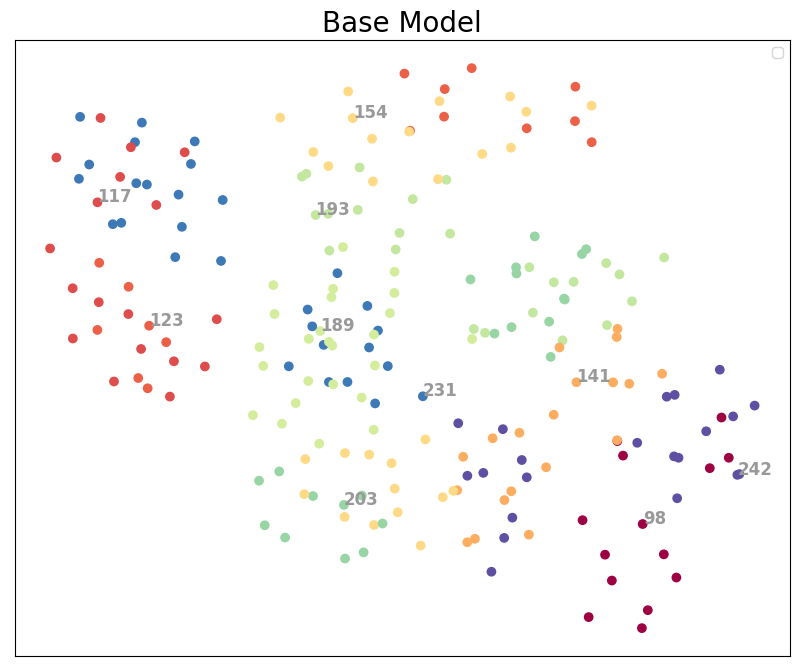
\includegraphics[width=0.42\linewidth]{t-SNE_68.55.png}}
  \subcaptionbox{\label{fig:tSNEb}}
    {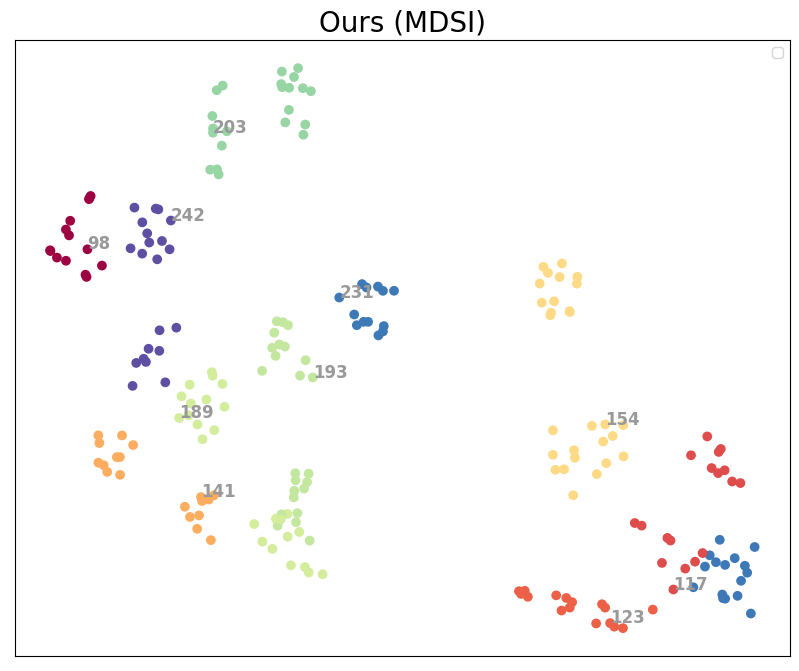
\includegraphics[width=0.42\linewidth]{t-SNE_75.07.png}}
  \subcaptionbox{\label{fig:confuse_base}}
    {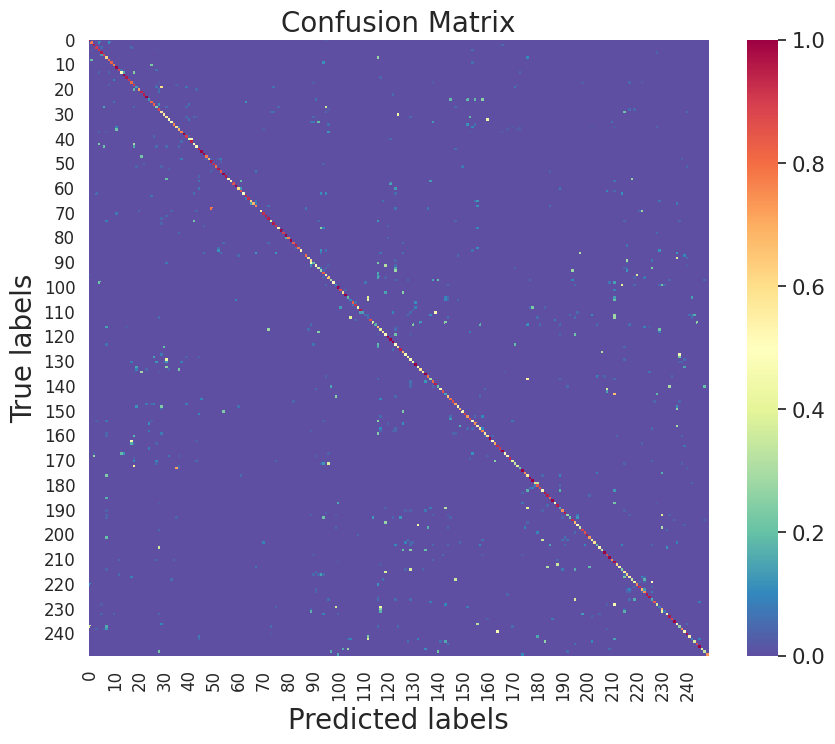
\includegraphics[width=0.49\linewidth]{confusion_matrix_59.85_spec.png}}
  \subcaptionbox{\label{fig:confuse_ours}}
    {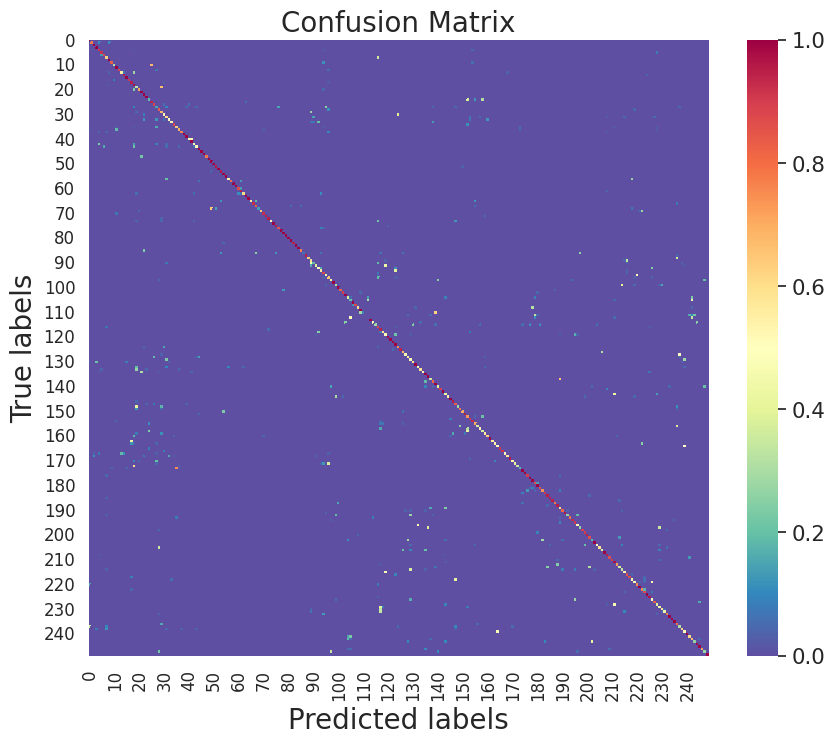
\includegraphics[width=0.49\linewidth]{confusion_matrix_75.07_spec.png}}
  \caption{可视化所提方法的增强效果。 (a) 基础模型的特征分布可视化。(b) 所提出的 MDSI 的特征分布可视化。(c) 基础模型的混淆矩阵。(d) 所提出的 MDSI 的混淆矩阵。}
  \label{fig:vis}
\end{figure}

\begin{figure}
  \centering
  \subcaptionbox{\label{fig:comp_gap}}
    {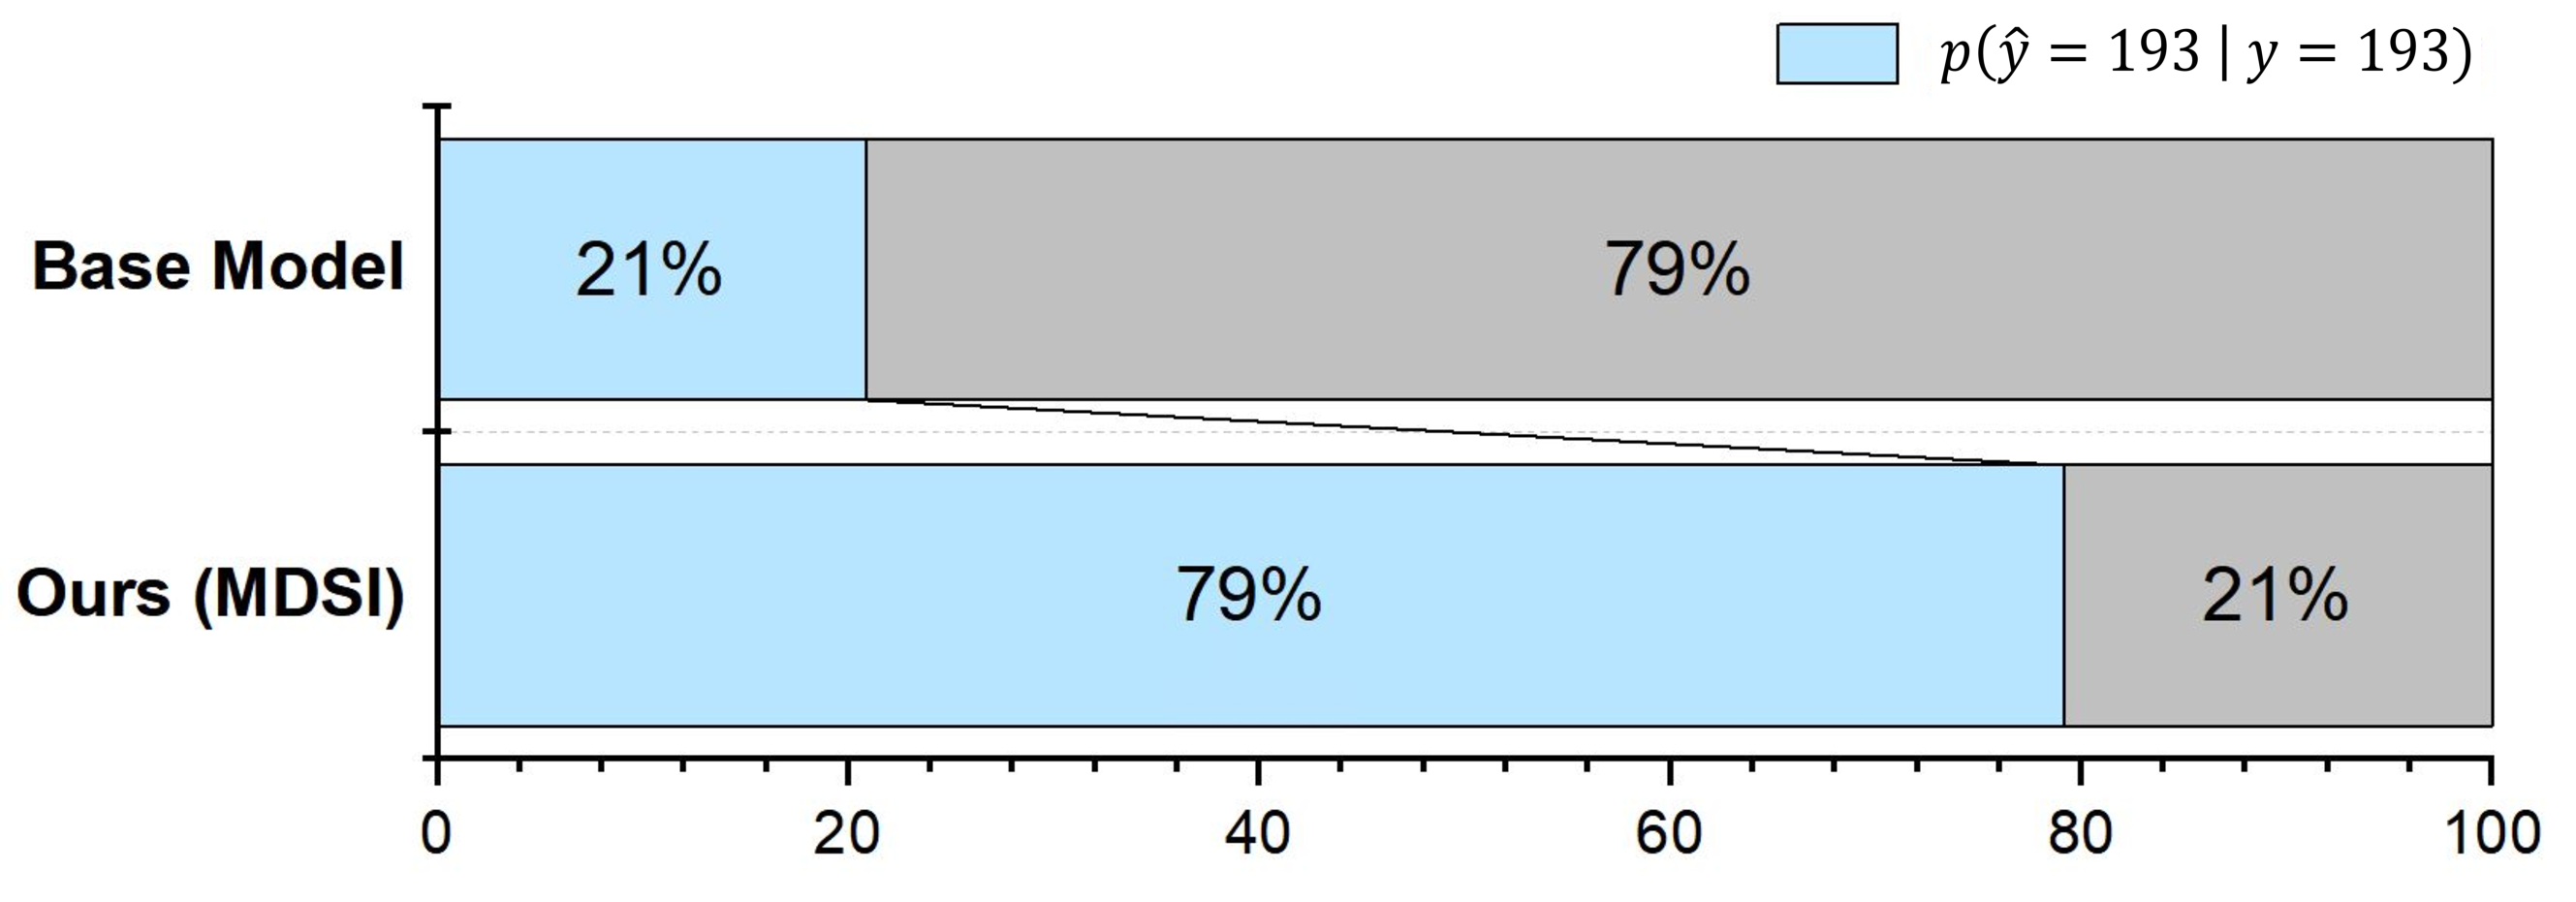
\includegraphics[width=0.49\linewidth]{comp_gap.pdf}}
  \subcaptionbox{\label{fig:comp_sim}}
    {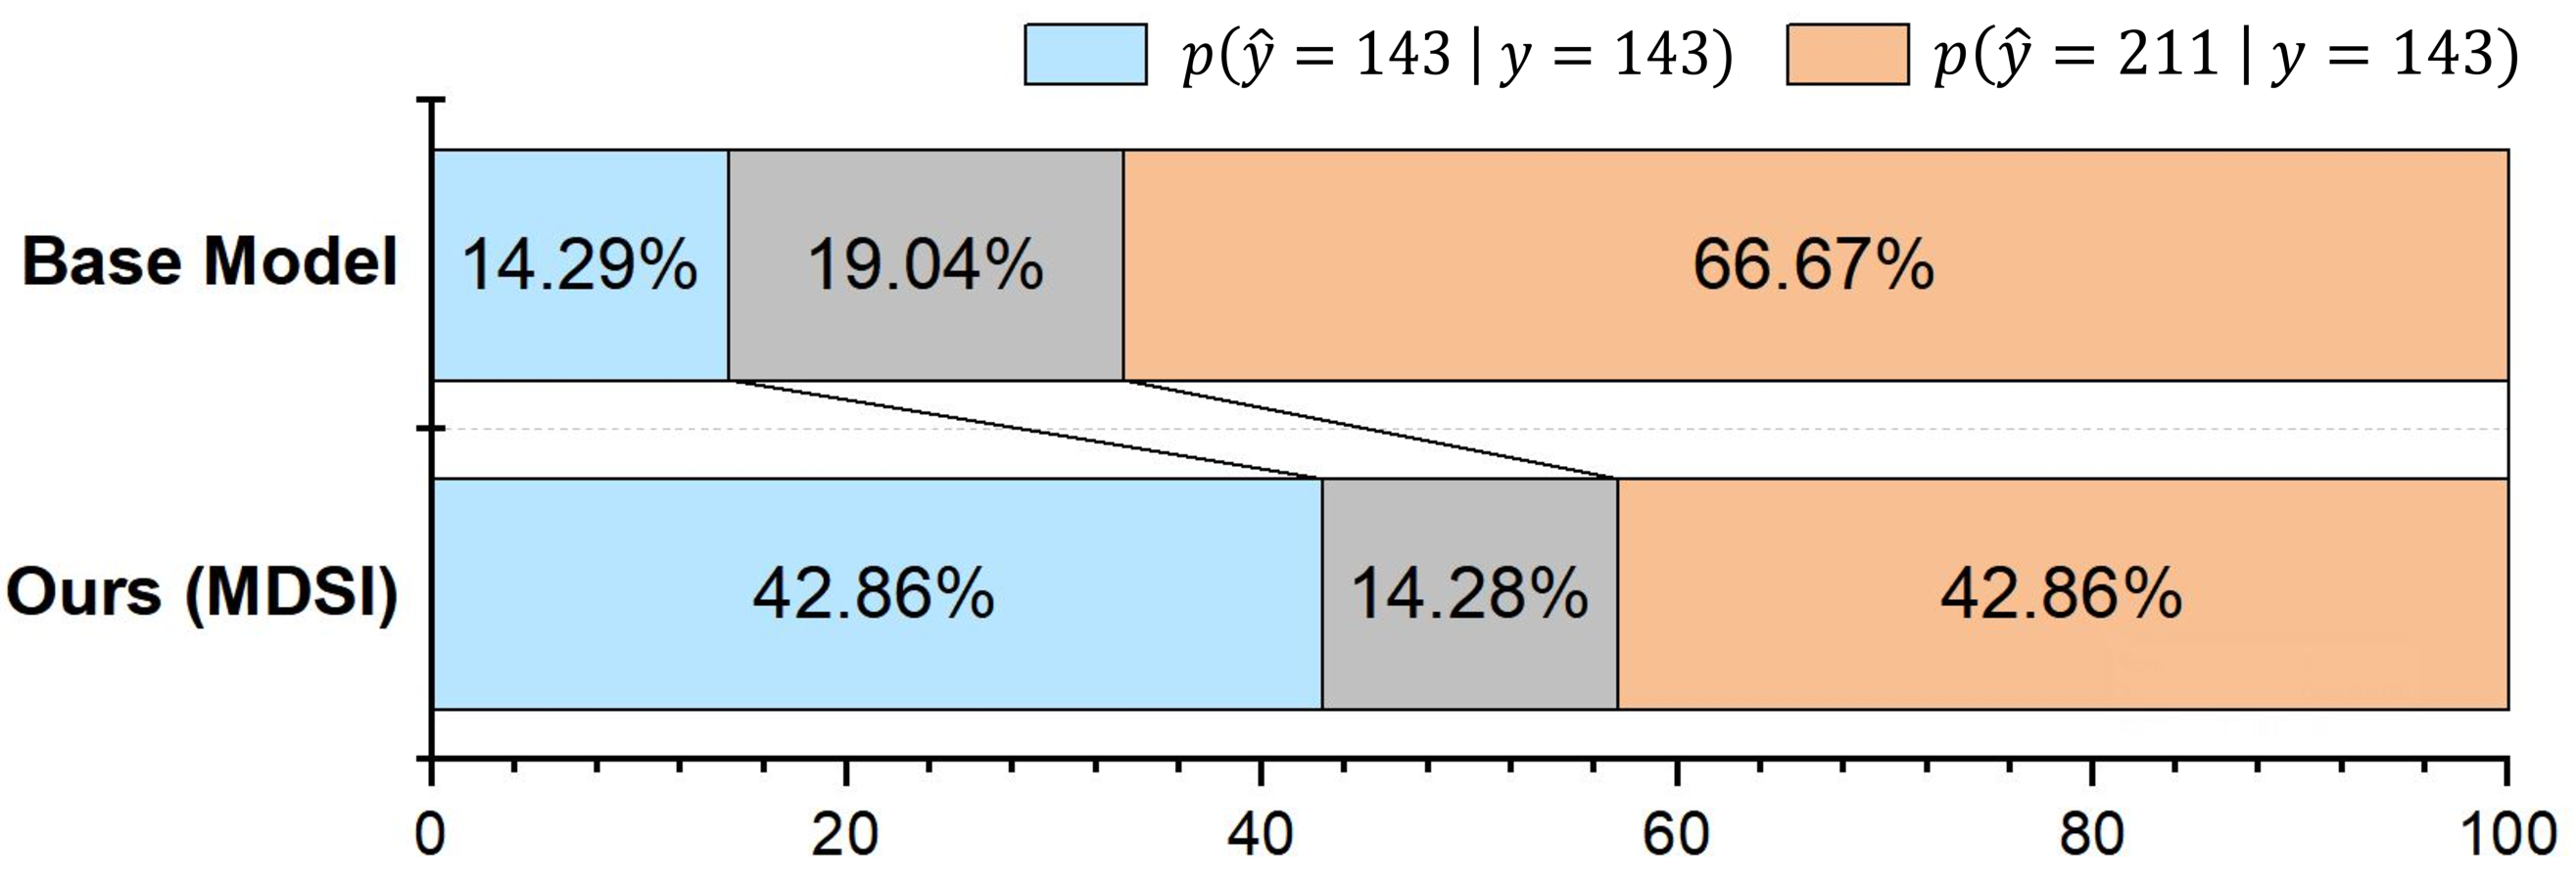
\includegraphics[width=0.49\linewidth]{comp_similar.pdf}}
  \caption{阐明所提出的 MDSI 在解决信息冗余 (IR) 和信息缺失 (IA) 挑战方面的增强功能。 (a) IR 场景下的性能改进(对应于图 ~\ref{fig:gap_sample} 中的样本)。 (b) IA 场景下的性能改进。(对应于图 ~\ref{fig:sim_sample} 中的样本)}
  \label{fig:comp}
\end{figure}

\subsubsection{定量和可视化结果}
为了进一步阐明我们方法的有效性,我们在图~\ref{fig:vis}中展示了 t-SNE 可视化和混淆矩阵。
此外,我们在图~\ref{fig:comp}中提供了统计结果,以突出 MDSI 在解决信息冗余 (IR) 和信息缺失 (IA) 挑战方面的改进。

在图~\ref{fig:tSNEa} 和 \ref{fig:tSNEb} 中,我们展示了基础模型和我们提出的 MDSI 方法的 t-SNE 可视化。
我们评估了与基础模型相比准确率提高最大的 10 个最具挑战性的类别。
基线模型 (图~\ref{fig:tSNEa}) 的视觉模式以相互交织的类别表示为特征,与我们的 MDSI (图~\ref{fig:tSNEb}) 实现的良好分离的聚类形成鲜明对比,这表明我们的 MDSI 有效地增强了特征表示的判别能力。
在图~\ref{fig:confuse_base} 和 \ref{fig:confuse_ours} 中,我们展示了基线模型和我们提出的 MDSI 的混淆矩阵。
矩阵显示,使用我们的方法,错误分类明显减少,说明了它通过最小化无关信息干扰来应对手势识别复杂性的卓越能力。
这种增强表明,所提出的方法不仅有效地增强了识别的鲁棒性和泛化能力,而且还增强了模型对关键手势特征的感知。

同时,我们对模型在信息冗余(IR)和信息缺失(IA)场景下的性能提升进行了详细分析。
考虑了图\ref{fig:samples}中描绘的两类样本对,图\ref{fig:comp_gap}和图~\ref{fig:comp_sim}分别说明了所提方法的影响。
MDSI带来的改进值得注意:i)对于遭受IR的样本类别,MDSI将准确率提高了58\%;ii)对于遭受IA的样本类别,MDSI将准确率提高了28.57\%,并将视觉相似类别的误分类率降低了23.81\%。
这些示例表明,我们的MDSI显着减轻了IR和IA对手势识别的影响,确保了稳健和通用的性能。


\section{本章小结}
本章提出了一种可插拔的多模态动态手势识别算法,称为多策略解耦与语义集成(MDSI),旨在解决RGB-D手势识别中的信息冗余(IR)和信息缺失(IA)挑战。
首先,第~\ref{sec:MDN}节引入了多策略解耦网络(MDN),通过解耦"姿态-运动"和"时空-通道"特征来减轻冗余信息。
随后,第~\ref{sec:SIN}节提出了语义集成网络(SIN),该网络通过语义过滤和标签平滑增强语义理解,有效地指导视觉相似手势的区分。
MDSI的可插拔特性使其能够以最小的计算开销无缝集成到各种视频编码器架构中,展示了其在动作识别和手语识别等相关领域的扩展潜力。大量实验(第~\ref{sec:GR_EXP}节)表明,MDSI在两个广泛认可的基准测试中超越了先前的最先进方法。
% 我们预计通过进一步改进MDSI和优化预处理将增强其实时部署能力。


% 理论依据:部分属于SOTA方法的有机结合

% \subsection{现阶段实验结果与讨论}
% \subsubsection{实验设置}
% 现阶段实验主要围绕GRGB分支(图\ref{fig:多流解耦注意力手势识别网络})展开,我们基于所提出的循环手势识别变换器(RGRT,图\ref{fig:RGRT})搭建了GRGB分支,并进行了一系列实验以验证RGRT在手势时空建模方面的有效性。
% 我们在大规模孤立手势数据集Jester-V1~\cite{jester2017}上进行预训练,并基于 ChaLearn LAP 孤立手势数据集IsoGD\cite{wan2016chalearn} 评估我们的动态手势识别算法。
% \paragraph{Jester数据集}~\cite{jester2017}。Jester是大量带有密集标签的视频剪辑的集合,是目前最大的孤立手势数据集。每个剪辑都包含工作人员在笔记本电脑摄像头或网络摄像头前执行的预定义手势。该数据集包含 27 种手势的 148094 个 RGB 视频文件,其中每个类别平均有超过 5000 个实例。
% \paragraph{IsoGD数据集}\cite{wan2016chalearn}。ChaLearn LAP RGB-D 孤立手势数据集(IsoGD)是一个用于手势识别的大型多模态数据集。该数据集包含 21 个不同个体执行的 249 个手势标签,共计47933个RGB-D手势视频实例。IsoGD由Microsoft Kinect传感器记录,包括传感器提供的RGB和Depth视频序列。
% \begin{figure}
%   \centering
%   \subcaptionbox{手势ID:50\label{fig:sa}}
%     {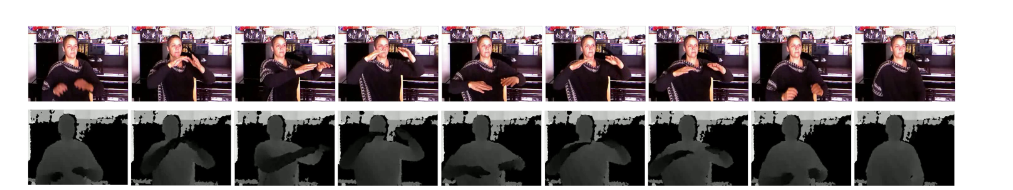
\includegraphics[width=0.75\linewidth]{samplesa.png}}
%   \subcaptionbox{手势ID:138\label{fig:sb}}
%     {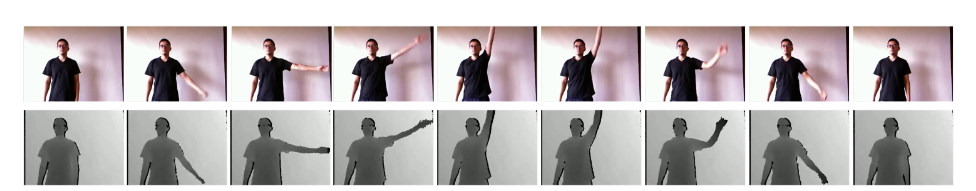
\includegraphics[width=0.75\linewidth]{samplesb.png}}
%   \caption{IsoGD\cite{wan2016chalearn}数据集动态手势样本示例}
%   \label{fig:samples}
% \end{figure}

% % AUTSL手语数据集。
% \subsubsection{RGRT效果分析} % 报告Jester和IsoGD
% 我们分别构建了基于所提出的循环手势识别变换器(RGRT)和基于不含变换器的循环模型的GRGB分支,并进行了对比实验。如表\ref{tab:ablation}结果所示,RGRT能够有效提升动态手势识别的准确率。这是由于RGRT网络巧妙地将循环结构与局部时域变换器(TWT)有效地结合,实现了多尺度时空建模。
% \begin{table}
%   \centering
%   \caption{GRGB分支消融分析}
%   \begin{tabular}{ccc}
%     \toprule
%     \multirow{2}{*}{Model} & \multicolumn{2}{c}{Accuracy(\%)}\\
%  & Jester\_val  & IsoGD\_val \\
%     \midrule
%     -w/o RGRT   & 93.60 & 55.71\\
%     Ours    & 94.07 & 56.67 \\
%     \bottomrule
%   \end{tabular}
%   \label{tab:ablation}
% \end{table}


% \subsubsection{与SOTA方法的比较} % 目前对比不使用额外通道的方法 % 报告IsoGD上的对比
% 我们将包含RGRT的GRGB分支网络与最先进的端到端手势识别网络进行了比较(如表\ref{tab:comparison}所示)。在IsoGD验证集上,我们的方法在RGB模态上取得了第二名的具有竞争力的识别性能,实现了56.67\%的准确率。仅略低于Zhu等人的方法\cite{zhu2019redundancy}(-0.75\%)。这可能是由于Zhu等人在汇报最终结果时使用了金字塔策略\cite{zhu2016large},对同一手势视频划分多段并融合预测。在后续工作中,我们计划对齐相关输入预处理技术,以更全面地比较模型性能。
% 上述实验结果突显了我们提出的包含RGRT的GRGB分支网络在手势时空建模方面的有效性,为后续解耦手势识别的研究打下了基础。
% \begin{table}
%   \centering
%   \caption{GRGB分支在IsoGD验证集上与SOTA方法的比较}
%   \begin{tabular}{lc}
%     \toprule
%     Method & Accuracy(\%)\\
%     \midrule
%     ResNet50\cite{narayana2018focus} & 33.22 \\
%     Pyramidal C3D\cite{zhu2016large}  & 36.58 \\
%     32-frame C3D\cite{li2016large} & 37.30 \\
%     8-MFFs-0f1c\cite{kopuklu2018motion} & 41.30 \\
%     Res3D\cite{miao2017multimodal} & 45.07 \\
%     3DCNN+BiConvLSTM+2DCNN\cite{zhang2017learning} &  51.31 \\
%     Res3D+ConvLSTM+MobileNet\cite{zhu2018continuous}  & 52.01 \\
%     ConvLSTMForGR\cite{zhu2019redundancy} & 55.98 \\
%     ConvLSTMForGR+Pyramid\cite{zhu2019redundancy} & 57.42 \\
%     \midrule
%     Ours -w/o RGRT & 55.71 \\
%     Ours & 56.67    \\
%     \bottomrule
%   \end{tabular}
%   \label{tab:comparison}
% \end{table}

% \subsubsection{推理速度}
% 我们在单张RTX2080显卡上对GRGB分支模型进行了推理速度测试,对同一样本进行了五次测试。如图\ref{fig:time}所示,GRGB分支的平均推理时间为83.9ms,快于范等人\cite{范桂双2020基于S3D}所公布的96ms。这表明我们的网络具有高效的推理能力。我们计划在后续工作中进一步优化网络结构,以进一步提升模型的推理速度。

% \begin{figure}
%   \centering
%   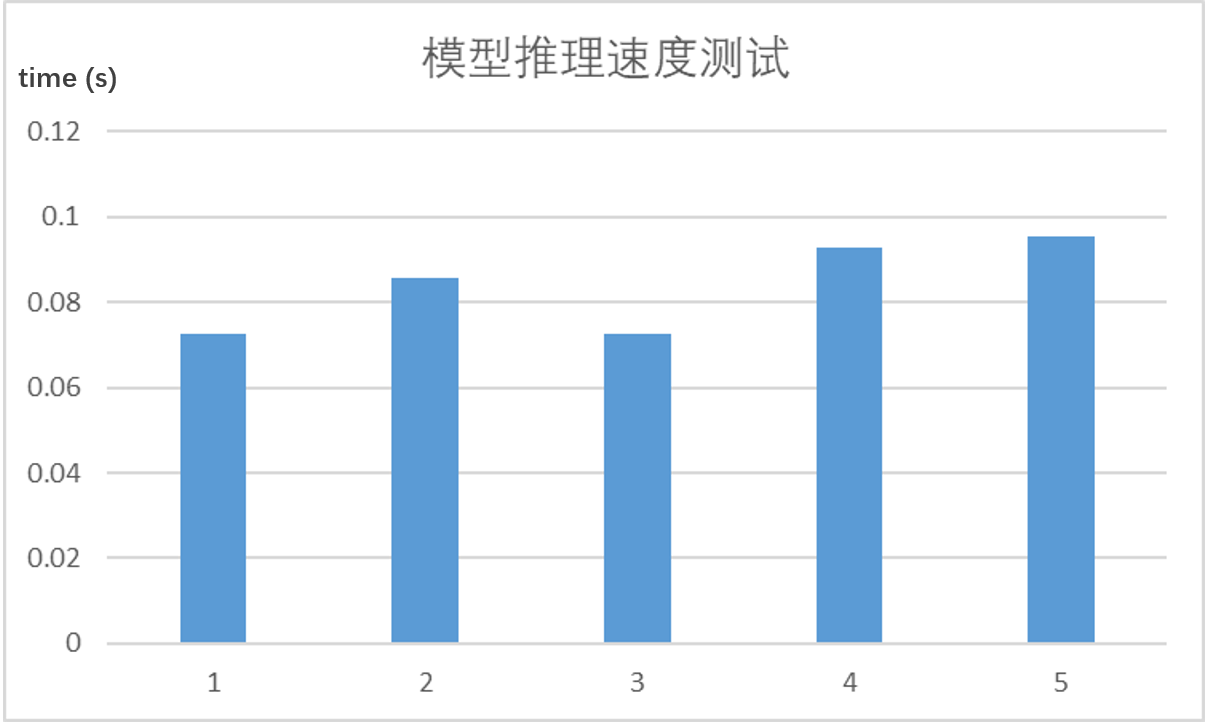
\includegraphics[width=0.65\linewidth]{time.png}
%   % \caption*{}
%   \caption{GRGB分支模型推理时间(单位:s)}
%   \label{fig:time}
% \end{figure}

% \subsubsection{解耦手势数据处理}
% 本研究使用HRNet\cite{sun2019deep}在上述数据集上事先提取并保存二维骨架数据(如图\ref{fig:8b}),随后进行手势解耦。目前,我们已经完成了Jester数据集上的解耦手势数据处理,后续将基于此开展解耦识别网络实验。
